%%% Dateikodierung: UTF-8
%%% äöüÄÖÜß  <-- keine deutschen Umlaute hier? UTF-faehigen Editor verwenden!

%%% Magic Comments zum Setzen der korrekten Parameter in kompatiblen IDEs
% !TeX encoding = utf8
% !TeX program = pdflatex 
% !TeX spellcheck = de_DE
% !BIB program = biber

\documentclass[bachelor,german,smartquotes]{hgbthesis}
% Zulässige Optionen in [..]: 
%    Typ der Arbeit: 'diploma', 'master' (default), 'bachelor', 'internship' 
%    Hauptsprache: 'german' (default), 'english'
%    Option zur Umwandlung in typografische Anführungszeichen: 'smartquotes'
%    APA Zitierstil: 'apa'
%%%-----------------------------------------------------------------------------

\RequirePackage[utf8]{inputenc} % bei Verw. von lualatex oder xelatex entfernen!

\graphicspath{{images/}}  % Verzeichnis mit Bildern und Grafiken
\logofile{logo}           % Logo-Datei: images/logo.pdf (kein Logo: \logofile{})
\bibliography{references} % Biblatex-Literaturdatei (references.bib)

%%%-----------------------------------------------------------------------------
% Angaben für die Titelei (Titelseite, Erklärung etc.)
%%%-----------------------------------------------------------------------------

% \title{toya\\ Imperative Programmiersprache für die JVM}
% \author{Lukas Christian Hofwimmer}
% \programname{Universal Computing}

%\programtype{Fachhochschul-Bachelorstudiengang} % auswählen/editieren
% \programtype{Fachhochschul-Bachelorstudiengang}

% \placeofstudy{Hagenberg}
% \dateofsubmission{2021}{07}{15} % {YYYY}{MM}{DD}

% \advisor{FH-Prof. DI Dr. Heinz Dobler} % optional

%\strictlicense % restriktive Lizenz anstatt Creative Commons (nicht empfohlen!)

%%%-----------------------------------------------------------------------------
\begin{document}
%%%-----------------------------------------------------------------------------

%%%-----------------------------------------------------------------------------
\frontmatter                                       % Titelei (röm. Seitenzahlen)
%%%-----------------------------------------------------------------------------

% \maketitle
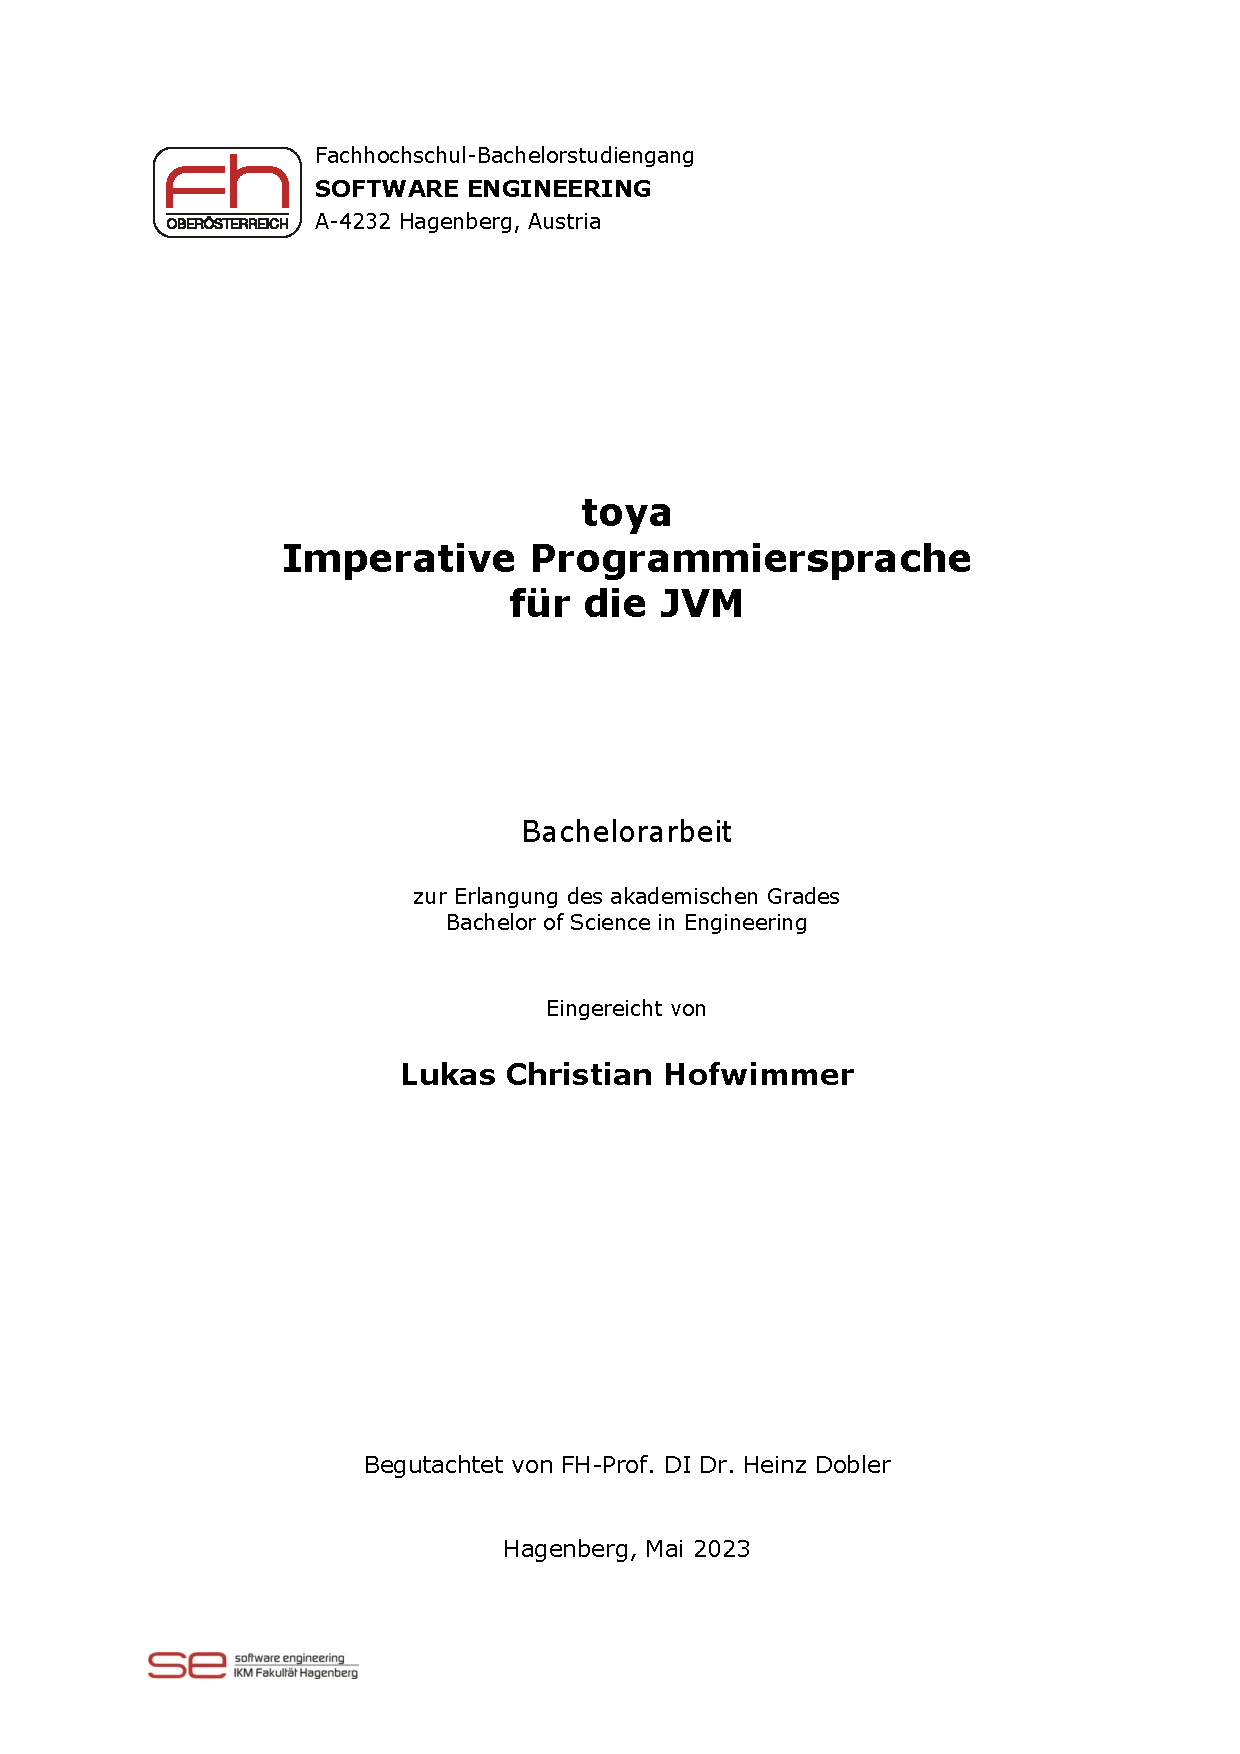
\includepdf[pages=1]{Titelblatt_Bachelorarbeit.pdf}
\includepdf[pages=2, pagecommand={\thispagestyle{empty}}]{Titelblatt_Bachelorarbeit.pdf}
\tableofcontents

\chapter{Vorwort}

 % Ein Vorwort ist optional
\chapter{Kurzfassung}

\Toya ist eine stark typisierte, turing\-vollständige Programmiersprache für die \textit{Java Virtual Machine} (JVM). \Toya erlaubt die Erstellung von Funktionen, Variablen, arithmetischen Ausdrücken und primitiven Kontrollstrukturen in Form von if-Verzweigungen und for-Schleifen.

Variablen können vom Typ \texttt{int}, \texttt{double}, \texttt{string} oder \texttt{boolean} sein. Ebenso ist es möglich, Felder dieser Typen anzulegen. Die explizite Angabe des Variablentyps ist mit Ausnahme von Feldern nicht möglich. Stattdessen ermittelt \toya anhand des zugewiesenen Ausdrucks den Typ der Variable.

Der Compiler für \toya ist in zwei Teile zu unterteilen: Frontend und Backend. Das Frontend kümmert sich um die Verarbeitung des Quelltext um daraus einen abstrakten Syntaxbaum zu erzeugen. Das Backend erzeugt anschließend anhand des abstrakten Syntaxbaum Bytecode für die JVM. Als Produkt liefert \toya class-Dateien, die die JVM verarbeitet und auswertet. Der Compiler für \toya ist vollständig in Kotlin/JVM implementiert.

Das Frontend verwendet als zentrale Bibliothek ANTLR in der vierten Version. ANTLR ist ein Parser-Generator, der anhand einer Grammatik-Datei, die die Struktur von \toya beschreibt, einen Parser in Form des Visitor-Entwurfsmuster erzeugt. Anhand dieses generierten Parsers durchläuft \toya den umfangreichen von ANTLR erzeugten Syntaxbaum und liefert einen abstrakten Syntaxbaum, der unter anderem nun Typinformationen besitzt. Mithilfe des Typsystem von Kotlin unterscheidet das Backend anschließend zwischen den verschiedenen Strukturen von \toya.

Das Backend verwendet als zentrale Bibliothek ObjectWeb ASM zum Generieren von Bytecode und class-Dateien. Als erstes erzeugt \toya eine einzelne Klasse \texttt{Main}, in welcher alle Funktionen eines \toya Programms liegen. Selbst, wenn ein \toya Programm über mehrere Dateien verteilt ist, erzeugt der Compiler nur eine class-Datei. Anschließend durchläuft das Backend den abstrakten Syntaxbaum. Jede Klasse des abstrakten Syntaxbaums besitzt eine Generierungs-Funktion, die den richtigen Bytecode für den Knoten des abstrakten Syntaxbaum erzeugt. Sobald der abstrakte Syntaxbaum fertig durchlaufen ist, erzeugt \toya eine ausführbare class-Datei.		
\chapter{Abstract}


\begin{english} %switch to English language rules
This should be a 1-page (maximum) summary of your work in English.
%und hier geht dann das Abstract weiter...
\end{english}

			

%%%-----------------------------------------------------------------------------
\mainmatter                             % Hauptteil (ab hier arab. Seitenzahlen)
%%%-----------------------------------------------------------------------------

\chapter{Einleitung}
\label{cha:Einleitung}

Compiler sind ein essenzieller Grundstein der Informatik und stellen das Bindeglied zwischen Mensch und Maschine dar. Erst durch sie wird die Entwicklung von höheren Programmiersprachen und Programmen einer Größenordnung möglich, die unsere moderne Welt im 21. Jahrhundert abverlangt. Ohne Compiler wäre die kommerzielle Entwicklung von Software unvorstellbar. Sie sind eine logische Schlussfolgerung, aus der Not gedrungen heraus immer effizienter werdende Anwendungen zu entwickeln. So weit, dass die Anweisungen an den Computer als lesbares Englisch verstanden werden kann. Im Zeitalter der kollaborativen Entwicklung gilt es, Programme nicht nur zu schreiben, sondern auch für sich selbst und Kolleg:innen lesbar zu machen. All diese Aspekte laufen darauf hinaus, dass Compiler die einzige Lösung sind.

Dementsprechend ist es Elementar, die Funktionsweise und Abläufe von Compilern zu verstehen. Der beste Weg, um dies zu bewerkstelligen, ist einen Compiler selbst zu schreiben.

\section{Zielsetzung}

Ziel dieser Arbeit ist es, eine neue Programmiersprache und einen entsprechenden Compiler dafür zu entwickeln. Dieser Compiler erzeugt Bytecode für die Java Virtual Machine, um \toya-Programme anschließend plattformunabhängig ausführen zu können. \Toya soll die Definition von Funktionen, primitiven Variablen und Feldern und Kontrollflüssen in Form von Verzweigungen und Schleifen erlauben. Daraus ergibt sich eine Turing-vollständige Programmiersprache, aus welcher heraus theoretisch alle anderen Programmiersprachen entstehen könnten. \Toya orientiert sich syntaktisch an Programmiersprachen wie C und Java mit einem Fokus auf Simplizität.

\section{Wieso die JVM?}

Eine grundsätzliche Frage, die es vor der eigentlichen Arbeit zu beantworten galt, war ob das Kompilat des \toya Compilers Maschinencode direkt oder ein Zwischenprodukt in Form von Bytecode für eine virtuelle Maschine produzieren sollte. Während der native Ansatz mit Maschinencode den Vorteil der Ausführungsgeschwindigkeit bringt, kommt auch der Nachteil der Implementierungskomplexität des Compilers einher.

Virtuelle Maschinen hingegen bieten eine Abstraktionsschicht über Maschinencode und machen die Entwicklung eines Compilers daher wesentlich leichter. Das ermöglicht, den Fokus auf andere Aspekte, wie die Verarbeitung des Syntaxbaums und die Generierung des Bytecodes zu legen, was auch im Verlauf dieser Arbeit klar zu erkennen ist.

Damit wurde klar, dass eine virtuelle Maschine die Ausgabe des Compilers interpretieren sollte. Unklar war jedoch weiterhin, welche virtuelle Maschine das Ziel sein sollte. Aufgrund der Menge an verfügbaren Resourcen, beschränkte sich diese Entscheidung auf die Java Virtual Machine und Common Language Runtime. Zweiteres bringt einige Vorteile, wie zum Beispiel, dass Typinformationen generischer Typen zur Laufzeit erhalten bleiben. \Toya nutzt jedoch nur einen Bruchteil aller möglichen Eigenschaften, weswegen dies keine entscheidende Rolle bei der Entscheidungfindung spielte. Schlussendlich fiel die Entscheidung auf die Java Virtual Machine aufgrund von Familiarität damit, könnte jedoch ebenso mit der Common Language Runtime implementiert werden.

\section{Aufbau der Arbeit}

Die Arbeit beschäftigt sich zuerst mit den theoretischen Grundlagen von \toya und den Werkzeugen, denen \toya zugrunde liegt. Anschließend werden konkrete Implementierungsdetails präsentiert und die Funktionalität der Sprache anhand von Beispielen bewiesen.

Das Kapitel \textit{Programmiersprache toya} stellt die Spezifikation der Sprache dar und bietet eine abstrakte Beschreibung der von \toya, ohne jedoch auf Implementierungsdetails einzugehen. Anschließend kommt es im Kapitel "Vergleich mit Kotlin" zur Gegenüberstellung mit einer etablierten Programmiersprache. Hierbei wurde Kotlin gewählt, da es sich dabei um die Implementierungssprache des \toya-Compilers handelt. Die Kapitel "Generierung des Syntaxbaums" und "JVM und Bytecode" bieten eine theoretische Beschreibung von ANTLR und der JVM. Das Kapitel "Implementierung" geht auf Implementierungsdetails des Compilers ein und bietet konkreten Einblick in Architektur anhand von Codebeispielen und Diagrammen. "Tests" zeigt die Funktionalität von \toya anhand von konkreten Codebeispielen und deren Ausgaben.
\chapter{Programmiersprache toya}
\label{cha:toya}

\Toya ist eine stark typisierte, turing\-vollständige Programmiersprache für die \textit{Java Virtual Machine} mit einem Fokus auf Simplizität. Der Syntax ist, wie bei C\# oder Java, stark an C angelehnt. Auf die Syntax wird in diesem Kapitel bei der näheren Behandlung der einzelnen Komponenten der Sprache eingegangen. 

\begin{CJK}{UTF8}{ipxm}
Der Name \toya, in Anlehnung an Java und Kotlin, findet seinen Ursprung bei einer Insel. Dabei handelt es sich konkret um 洞爺湖 (Tōya-ko), einen Kratersee im Norden Japans, der wiederum die Insel 中島 (Nakajima) enthält. Von Tōya-ko leitet sich dann der Name \toya ab.
\end{CJK}

\Toya folgt dem imperativen Programmierparadigma. Ein \toya-Programm besteht aus einer Menge an Funktionen und Variablen, wobei wie in Java eine \texttt{main}-Funktion zum Programmeinstieg notwendig ist. Klassen gibt es keine. Bei der Übersetzung werden aber alle Programmteile in eine \texttt{Main} Klasse zusammengefasst, da das resultierende Kompilat mindestens eine Klasse benötigt. Sollte die \texttt{main} Funktion nicht vorhanden sein, so wird eine Ausnahmesituation während der Syntax-Analyse erzeugt. Variablen, die außerhalb von Funktionen definiert werden, stehen global zur Verfügung. Global in diesem Kontext bedeutet, dass solche Variablen in allen Funktionen des Programms verwendet werden können.

Die Benutzer:in hat die Möglichkeit, ein \toya-Programm auf mehrere Dateien aufzuteilen. Anschließend bei der Übersetzung sind alle \texttt{toya}-Dateien anzugeben. Unabhängig von der Anzahl an Eingangs-Dateien besteht das kompilierte Programm jedoch immer aus genau einer \texttt{class}-Datei.  

\section{Typen}

\Toya stellt insgesamt fünf Typen und Felder von diesen Typen zur Verfügung. Diese sind \texttt{boolean}, \texttt{int}, \texttt{double} und \texttt{string}. Die Auswahl der Typen beschränkt sich auf solche, die eindeutig unterschiedliche Aufgaben erfüllen. Das Erstellen weiterer Typen ist nicht möglich.

Feld-Typen sind mit dem allgemein bekannten Suffix \texttt{[]} und dem Schlüsselwort \textit{new} zu deklarieren. So ist zum Beispiel der Typ eines Zeichenketten-Feldes als \texttt{[]} zu schreiben.

Die JVM bietet zusätzlich noch die Datentypen \texttt{byte}, \texttt{short}, \texttt{long} und \texttt{float}. All diese Typen sind zwar für größere Programme relevant und notwendig, überschneiden sich aber und kommen in \toya daher nicht vor. Der Sinn von \toya ist nicht die vollständige Ausschöpfung aller JVM-Eigenschaften, sondern die explorative Implementierung einer Programmiersprache. Dafür sind nicht alle Datentypen notwendig. Der \texttt{returnAddress}-Typ wird hier außer acht gelassen, weil dieser nur JVM-interne Relevanz hat.

\texttt{int} hat einen Wertebereich von $-2^{31}$ bis $2^{31} - 1$; \texttt{double} folgt der IEEE-754-Spezifikation: 1 Bit für das Vorzeichen, 11 Bit für den Exponenten und 52 Bit für die Mantisse. \texttt{boolean} hat die Werte \texttt{true} und \texttt{false}. \texttt{True} wird intern als $1$ mit repräsentiert, \texttt{false} mit 0. Die JVM kennt keinen nativen Zeichenketten-Typ, da dieser als Referenz repräsentiert wird. Da \toya keine Erstellung von Typen erlaubt, sind die einzigen Referenztypen Zeichenketten und Felder. Die Bytecode-Generierung von \toya unterscheidet immer zwischen Felder und nicht-Felder, wenn es um die Auswahl der richtigen Opcodes geht. Daraus folgt, dass eine Referenz, welche kein Feld ist, immer eine Zeichenkette sein muss. Zeichenketten werden als Literale mit doppelten Anführungszeichen definiert. So ist ein Hello World String als \texttt{``Hello World''} anzugeben.

Sprachen wie Java oder Kotlin konvertieren automatisch zwischen Typen, wenn diese zum Beispiel in arithmetischen Operationen gemischt werden. So liefert eine Addition, mit einem Ganzzahl- und Gleitkomma-Operanten eine Gleitkomma-Summe. Dadurch ermöglichen diese Programmiersprachen eine gewisse Flexibilität, selbst bei statischer Typisierung. Diese automatische Konvertierung besitzt \toya nicht. Stattdessen wird das Programm in einen Ausnahmezustand versetzt, sollten verschiedene Typen in einer Operation vorkommen.

\section{Funktionen}

Funktionen sind die zentrale Komponente von \toya und enthalten die Programmlogik. Sie bestehen aus Funktionssignatur und Funktionskörper. Die Funktionssignatur besteht aus Funktionsname, Parameter und Rückgabewert. Der Name ist das einzig verpflichtende hierbei; Parameter und Rückgabewert sind optional. Hat eine Funktion keinen Rückgabewert, so entfallen der Pfeil und nachfolgende Typ. In~\autoref{lst:intro_simplefunction} ist eine eine einfache Funktion zu sehen, die zwei Ganzzahlen addiert und deren Summe zurückliefert.

\begin{ToyaCode}[numbers=none, caption={Eine typische Funktion unter toya.}, label=lst:intro_simplefunction]
function add(lhs: int, rhs: int) -> int {
    lhs + rhs
}
\end{ToyaCode}

Der Funktionskörper besteht aus einer beliebigen Folge an Anweisungen und Ausdrücken. Hat eine Funktion einen Rückgabewert, so kann mit \texttt{return} ein nachfolgender Ausdruck rückgegeben werden. Das Schlüsselwort \texttt{return} ist jedoch optional: Wenn die letzte Anweisung gleichzeitig ein Ausdruck und vom gefordertem Typen ist, dann wird automatisch dieser Ausdruck geliefert. Hierbei ist jedoch zu beachten, dass die Leserlichkeit erhalten bleibt.

Der Aufruf einer Funktion erfolgt mit dem Syntax \texttt{function <name>(parameters)}. Eine Funktion kann eine beliebig Menge an Parameter aufweisen. Für jeden Parameter kann jeder beliebige Ausdruck eingesetzt werden, solange der Formal- und Aktualtyp übereinstimmt.

% TODO Std Functions

\section{Variablen}
\Toya erlaubt Nutzer:innen die Erstellung von Variablen in Funktionen und auf globaler Ebene. Der Syntax dafür lautet \texttt{var <name> = <ausdruck>}; die explizite Angabe eines Typs ist nicht möglich. Stattdessen leitet der Compiler anhand bekannter Typinformation des zu evaluierenden Ausdrucks den Typ ab und weist diesen Typ der Variable zu. Dieser Typ bleibt über die gesamte Lebensdauer der Variable gleich. Sobald der Typ einer Variable fixiert ist, so kann er nicht mehr geändert werden. Initialisiert man also eine Variable mithilfe eines Ganzzahl-Ausdrucks, so ist die Variable bis dessen Speicherplatz durch die automatische Speicherplatzverwaltung freigegeben wird, vom Typ \texttt{int}. Eine getrennte Deklaration und Initialisierung ist nicht möglich.

Abgesehen von typentheoretischer Relevanz bietet die Verwendung des Schlüsselwortes \texttt{var} einige Vorteile aber auch Nachteile für Verwender:innen von \toya. Da \texttt{var} alle anderen Typen ersetzt, erleichtert es die Schreibarbeit für Programmierer:innen ungemein. Robert C. Martin sagt jedoch in seinem nominalen Werk \textcite{martin2009clean} ``Indeed, the ratio of time spent reading vs. writing is well over 10:1. We are constantly reading old code as part of the effort to write new code.''. Daraus folgt, dass die Lesbarkeit wichtiger als Schreibbarkeit von Code ist und hierbei zeigen sich die Schwächen. Mit nur einem Schlüsselwort kann der Typ einer Variablen nicht explizit angegeben werden und muss durch den Leser:in abgeleitet werden. Ergo ist die Lesbarkeit von \toya Code schlechter als bei anderen Sprachen. Um diesem Problem vorzubeugen bieten moderne Entwicklungsumgebungen Hinweise auf den Typ in der grafischen Benutzeroberfläche. Aufgrund der geringen Anzahl an Typen in \toya ist das Fehlen von Typhinweisen jedoch vernachlässigbar.

Vergleicht man nun die Variablendeklaration und Initialisierung von \toya~\ref{lst:intro_varinittoya} mit Java~\ref{lst:intro_varinitjava}, so ist zu erkennen, dass bei der Initialisierung via Literalen die Verwendung von \texttt{var} kein Problem darstellt. Will man einer Variable den gelieferten Wert einer Funktion zuweisen, so können hier aber Schwierigkeiten hinsichtlich Schlussfolgerungen auftreten. Daher ist die bewusste und intelligente Vergabe von Variablennamen essenziell.

\begin{ToyaCode}[numbers=none, caption={Variablendeklaration in toya}, label=lst:intro_varinittoya]
var number = 123
var word = "Hello World"
var value = 123.456
var bool = true
var result = someFunction()
\end{ToyaCode}

\begin{JavaCode}[numbers=none,caption={Variablendeklaration in Java (vor Version 10)}, label=lst:intro_varinitjava]
int number = 123;
String word = "Hello World";
double value = 123.456;
boolean bool = true;
int result = someFunction();
\end{JavaCode}

Der Name einer Variable darf nur einmal im Gültigkeitsbereich verwendet werden, da es ansonsten zu Unklarheiten kommen kann, welche von mehreren Variablen nun gemeint ist. Auf die Frage, was sich hinter einem Gültigkeitsbereich verbirgt, wird näher im Kapitel \ref{cha:implementation} eingegangen. Ein Name darf aus beliebig vielen Groß- und Kleinbuchstaben und Unterstrichen bestehen.

\subsection{Felder}

Ein Feld ist eine eindimensionale Folge eines bestimmten Typs mit einer fixen Länge, welche bei der Deklaration des Feldes angegeben wird und sich über die Lebensdauer des Feldes nicht mehr ändert. Zuweisungen und Deklarationen unterscheiden sich nur leicht von nicht-Feld Variablen. Der Hauptunterschied dabei besteht darin, dass die Länge bei der Deklaration und der Index bei der Zuweisung anzugegeben is.

Felder werden mit der Syntax \texttt{var <name> = new <typ>[int-Ausdruck]} deklariert. Mit \texttt{<name>[int-Ausdruck] = Ausdruck} wird ein neuer Wert auf die Speicheradresse, dies anhand des Index berechnet wird, geschrieben.

\section{Anweisungen}

Anweisungen sind Befehle, die keinen Wert liefern. Dazu gehören For-Schleifen und Return-Anweisungen.

\subsection{For-Schleifen}

For-Schleifen in \toya verhalten sich gleich wie in vielen anderen Sprachen. Sie bestehen aus einem Schleifenkopf und einem Schleifenkörper. Der Schleifenkopf besteht aus drei Teilen von denen alle drei optional sind:
\begin{itemize}
    \item \textbf{Zählvariable:} Eine Variablendeklaration.
    \item \textbf{Abbruchbedingung:} Ein Ausdruck, der zu einem booleschen Wert evaluieren muss. Solang dessen Wert \texttt{true} ist, läuft die Schleife.  
    \item \textbf{Inkrement-Ausdruck:} Der Ausdruck, welcher nach jedem Schleifendurchlauf evaluiert wird und typischerweise die Zählvariable verändert.
\end{itemize}

\begin{ToyaCode}[numbers=none, caption={Eine For-Schleife, die die Zählvariable auf die Konsole ausgibt.}]
for (var i = 0; i <= 10; i++) {
    println(i)
}
\end{ToyaCode}

Gibt es keine Abbruchbedingung, so läuft die Schleife, solange das Programm läuft. Wie in Java kann die Entwickler:in mit der Anweisung \texttt{for (;;) \{ ... \}} eine Endlos-Schleife erzeugen.

\section{Ausdrücke}

Alle Konstrukte, die einen Wert liefern, sind Ausdrücke in \toya. So sind Funktionsaufrufe, die einen Rückgabewert haben, If-Verzweigungen, boolesche und arithmetische Ausdrücke, Literale und Variablen Ausdrücke. Ausdrücke evaluieren immer zu einem Wert, welcher aus dem Wertebereich eines bestimmten Typs entstammt. Abgesehen vom zwingendem Übereinstimmen des Formal- und Aktualtyps existieren keine Beschränkungen, was das Ersetzen von Ausdrücke durch andere Ausdrücke betrifft.

\subsection{Arithmetik}

\Toya unterstützt Addition (\texttt{+}), Subtraktion (\texttt{-}), Multiplikation (\texttt{*}) und Division (\texttt{/}) für Ganzzahl- und Gleitkomma-Werte via Infix Notation. Bei der Evaluierung von arithmetischen Ausdrücken wird auf die Klammerung und auf die Operatorrangfolge Rücksicht genommen, sodass arithmetische Ausdrücke in der richtigen Reihenfolge evaluiert werden. 

% TODO precedence der Operatoren Grafik hier einfügen

\subsection{Boole'sche Logik}

Boole'sche Ausdrücke sind essenziell für die Verwendung von If-Verzweigungen und For-Schleifen, da sie für die Zweig-Wahl, beziehungsweise als Abbruchbedingung benötigt werden. Zur Auswahl stehen die boole'schen Operatoren \textit{Und} (\texttt{\&\&}) und \textit{Oder} (\texttt{||}) und die relationalen Operatoren Größer (\texttt{>}), Größer-Gleich (\texttt{>=}), Gleich (\texttt{==}), Kleiner-Gleich (\texttt{<=}) und Kleiner (\texttt{<}). Außerdem können booleäsche Ausdrücke mit dem Präfix \texttt{!} negiert werden. Es ist zu beachten, dass relationale Operatoren eine höhere Rangigkeit als boole'sche Operatoren haben, sodass selbst ohne richtiger Klammerung der Ausdruck auf die erwartete Weise evaluiert wird. Die Rangfolge der Operatoren hierbei entspricht der von C.

% TODO Tabelle welche Operation für welchen Typen unterstützt wird.

\subsection{If-Verzweigungen}

If-Verzweigungen ermöglichen Entwickler:innen, bedingte Ausführung zu implementieren. If-Verzweigungen sind sehr flexibel in ihrer Syntax, da sowohl ein einzelner Ausdruck, als auch ein Block mit mehrere Anweisungen in den Zweigen des Ifs angegeben werden kann. 

\texttt{if (<boolean-expression>) \{ <statement>* \} else \{ <statement>* \}} ermöglicht die Angabe von mehreren Anweisungen pro Block, wobei jeder Block von geschwungenen Klammern umgeben ist, wie in~\autoref{lst:intro_ifexpanded} zu sehen ist. Hat man die Absicht, nur einen Ausdruck pro Zweig anzugeben, dann reicht \texttt{if (<boolean-ausdruck>) expression else expression} völlig aus. Siehe~\autoref{lst:intro_ifexpression} dazu.

\begin{ToyaCode}[numbers=none, caption={If-Verzweigung als klassische Anweisung.}, label=lst:intro_ifexpanded]
var someBoolean = true
if (someBoolean) {
    doSomething()
    print(someBoolean)
} else {
    print(someBoolean)
}
\end{ToyaCode}

\begin{ToyaCode}[numbers=none, caption={If-Verzweigung als Ausdruck in einer Variablenzuweisung.}, label=lst:intro_ifexpression]
var someBoolean = false
var someInteger = if (someBoolean) 4 else 5
\end{ToyaCode}

Die Stärke der If-Verzweigung in \toya liegt darin, dass es nicht nur ein Anweisung ist, sondern auch die Verwendung als Ausdruck möglich ist. Dadurch kann eine If-Verzweigung auf der rechten Seite einer Variablenzuweisung, in arithmetischen Ausdrücken, als Bedingung in anderen If-Verzweigungen, etc. vorkommen. Andere Programmiersprachen, wie Java, bieten einen ternären Operator \texttt{var x = boolean-expression ? expression : expression}. Dieser existiert in \toya jedoch nicht, da die If-Verzweigung bereits diesen Zweck erfüllt. 

% TODO: Hinweis auf Kotlin
% https://discuss.kotlinlang.org/t/ternary-operator/2116/10
% short answer: https://discuss.kotlinlang.org/t/ternary-operator/2116/171

Um die Verwendung als Ausdruck zu ermöglichen, ist zu beachten, dass bei If-Verzweigungen mit Blöcken die letzte Anweisung ein Ausdruck sein muss. Handelt es sich um eine If-Verzweigungen mit Ausdrücken besteht jeder Zweig aus nur einem einzelnen Ausdruck. Dadurch ist diese Bedingung sowieso gegeben. Außerdem müssen die Typen in allen Zweigen übereinstimmen und der sonst optionale else-Zweig zwingend vorhanden sein. Wäre der else-Zweig nicht vorhanden, dann wäre unter Umständen kein Wert als Folge der Evaluierung gegeben.

\subsection{Literale}

Literale sind die primitivsten Ausdrücke in \toya und stellen fixe Werte dar. Jeder Typ hat ein bestimmtes Format für Literale, sodass Typ-Inferenz möglich ist. 

\begin{itemize}
    \item \textbf{int:} Alle numerischen Werte ohne Nachkommastellen. (z.B.: \texttt{12345})
    \item \textbf{double:} Alle numerischen Werte mit Nachkommastellen. (z.B.: \texttt{123.45})
    \item \textbf{string:} Zeichenketten, die von doppelten Anführungszeichen umgeben sind. (z.B.: \texttt{``Hello World''})
    \item \textbf{boolean:} \texttt{true} und \texttt{false}. 
\end{itemize}

\section{Kommentare}

\toya erlaubt die Verwendung von Kommentaren. Ein Kommentar beginnt mit einem doppelten Schrägstrich \texttt{//}; alle weiteren Zeichen in dieser Zeile -- bis zum Zeilenumbruch -- ignoriert der Parser.
\chapter{Vergleich mit Kotlin}
\label{cha:comparison}

Da der \toya Compiler in Kotlin impelementiert und die Syntax auch an Kotlin angelehnt ist liegt es nahe, einen Vergleich zwischen den beiden Sprachen durchzuführen. Ein besonderer Fokus im Vergleich liegt auf der Syntax, da der generierte Bytecode zwischen den beiden Sprachen kaum zu unterscheiden ist (abgesehen von Optimierungen für individuelle Code-Stücke in Kotlin). Im Folgenden werden nur die wesentlichen Unterschiede zwischen den beiden Sprachen im Kontext von \toya aufgezeigt. Im Sinne der Prägnanz wird über den direkten Vergleich hinaus nicht näher auf Kotlin eingegangen. Zum Vergleich mit Kotlin wird die offizielle Kotlin Dokumentation von Jetbrains verwendet \parencite{kotlindocs}.

\section{Übersicht Kotlin}
Kotlin ist eine seit 2011 entwickelte statisch typisierte, imperative Programmiersprache mit Elementen der funktionalen Programmimerung. Als Antwort von JetBrains auf Java und Scala bietet Kotlin eine plattformübergreifende und idiomatische Programmiersprache, welche nahtlos in das JVM Ökosystem eingegliedert ist. Neben der JVM übersetzt Kotlin auch zu JavaScript, WebAssembly und Assembly. Für letzteres verwendet Kotlin die Compiler-Infrastruktur LLVM. Das momentane Haupt-Anwendungsgebiet liegt in der mobilen Entwicklung unter Android.

%  TODO: Google I/O 2019 reference https://developer.android.com/kotlin/first
Google empfiehlt seit 2019 Kotlin anstatt Java zu verwenden und bietet Teile der Standardbibliothek - Jetpack Compose - nur noch unter Kotlin an, da hierbei der Einsatz von Kotlin-spezifischen Compiler Plugins notwendig ist \parencite{kotlinfirst}. Andrey Breslav leitete bis 2020 die Entwicklung von Kotlin und übergab anschließend die Verantwortung an Roman Elizarov. Aktuell befindet sich Kotlin bei der Version 1.8.21.

Eines der wichtigsten Merkmale von Kotlin ist die Vermeidung des \textit{Billion Dollar Mistake}: Null Pointer. Indem der Compiler bei der unerlaubten Zuweisung von Null-Werten in einen Ausnahmezustand versetzt wird, kommen während der Laufzeit wesentlich weniger \texttt{NullPointerException} zustande. Da es jedoch weiterhin Fälle gibt, in welchen \texttt{null} ein erwünschter Wert ist, kann die Entwickler:in via \texttt{?} den Typ einer Variable als \textit{nullable} markieren.

Ein weiteres wichtiges Ziel Kotlins ist die Lesbarkeit des Codes. Dies zeigt sich vor allem in den Methoden der Standardbibliothek. So gibt es zum Überprüfen von Listen auf deren Leerheit die Methode \texttt{isEmpty()}, aber auch dessen Negation mit \texttt{isNotEmpty()}. Diese zweite Methode ist redundant, erleichtert aber die Lesbarkeit des Codes.

Hinsichtlich der funktionalen Programmierung bietet Kotlin eine leicht verwendbare Syntax an, um zum Beispiel die Komposition von Funktionen umzusetzen. Unter anderem stehen Funktionen höherer Ordnung, Lambdafunktionen und Erweiterungsfunktionen zur Verfügung. Diese finden auch häufig Verwendung in der Standardbibliothek: \textit{Scope functions} sind Funktionen höherer Ordnung, die auf ein Objekt eine Lambdafunktion anwenden. Konkret stehen \texttt{let}, \texttt{run}, \texttt{with}, \texttt{apply} und \texttt{also} zur Verfügung, welche sich in der Art und Weise, wie sie das Objekt behandeln, unterscheiden. Auf diese Funktionen wird nicht näher eingegangen, da diese nicht Teil dieser Bachelorarbeit sind.

\section{Funktionen}

Kotlin verwendet das Schlüsselwort \texttt{fun} zur Funktionsdefinition. Der Programmeinstieg geschieht über eine eindeutig identifizierbare \texttt{main}-Funktion, welche man optional mit einem \texttt{args: String[]} Parameter versehen kann. Entscheidet die Benutzer:in sich dazu, die \texttt{main}-Funktion parameterlos zu implementieren, erstellt der Compiler intern eine zweite \texttt{main}-Funktion mit \texttt{args: String[]} Parameter, welche dazu dient, die, von der Nutzer:in definierte \texttt{main}-Funktion aufzurufen. Wie in~\autoref{lst:cmp_kotlinfunction} und~\autoref{lst:cmp_toyafunction} zu sehen ist, gleichen sich \toya und Kotlin, abgesehen von kleinen syntaktischen Unterschieden.

\begin{KotlinCode}[numbers=none, caption={Funktion unter Kotlin}, label=lst:cmp_kotlinfunction]
fun add(lhs: Int, rhs: Int) : Int {
    return lhs + rhs
}
\end{KotlinCode}

\begin{ToyaCode}[numbers=none, caption={Funktion unter \toya}, label=lst:cmp_toyafunction]
function add(lhs: int, rhs: int) -> int {
    return lhs + rhs
}
\end{ToyaCode}

\section{Variablen}

In Kotlin stehen zur Deklaration von Variablen die Schlüsselwörter \texttt{var} (Wert ist veränderbar) und \texttt{val} (Wert ist unveränderbar) zur Verfügung. Die Bestimmung des Typs erfolgt entweder implizit anhand des zugewiesenen Ausdrucks oder explizit.\\ \texttt{val someString: String = ``Hello World''} weist der Variable \texttt{someString} den Wert \textit{Hello World} zu. Die explizite Angabe des Typs \texttt{String} ist bei diesem Beispiel redundant, da aus dem Ausdruck der Typ ableitbar ist.~\autoref{lst:cmp_kotlinvariables} zeigt die Initialisierung von drei Variablen mit expliziter und zwei weitere Variablen mit impliziter Typangabe in Kotlin.

Im Gegensatz dazu bietet \toya nur das Schlüsselwort \texttt{var} zur Variablendeklaration an, da in \toya alle Variablen veränderbar sind. Die explizite Angabe von Typen ist nicht möglich. Der Typ leitet sich immer vom Ausdruck ab.~\autoref{lst:cmp_toyavariables} zeigt die Initialisierung der selben Variablen mit den selben Werten wie in~\autoref{lst:cmp_kotlinvariables} mit dem Unterschied, dass diese in nun in \toya implementiert sind.

\begin{KotlinCode}[numbers=none, caption={Variablendeklarationen in Kotlin}, label=lst:cmp_kotlinvariables]
val number: Int = 123
val word: String = "Hello World"
var value: Double = 123.456
var bool = true
var result = someFunction()
\end{KotlinCode}

\begin{ToyaCode}[numbers=none, caption={Variablendeklarationen in \toya}, label=lst:cmp_toyavariables]
var number = 123
var word = "Hello World"
var value = 123.456
var bool = true
var result = someFunction()
\end{ToyaCode}

\section{Felder}

Kotlin bietet für die Verwendung von Feldern die generische Klasse \texttt{Array} an. Die Größer der Felder in Kotlin ist statisch. Daher ist die Anzahl an speicherbaren Elementen via Konstruktorparameter anzugeben. Alternativ dazu besteht die Möglichkeit, mit der Hilfs-Funktion \texttt{arrayOf} ein Feld mit Werten zu initialisieren, wie in~\autoref{lst:cmp_kotlinarrays} zu sehen ist. Für jeden primitiven Typ existiert eine eigene Feld-Klassen. \Toya hingegen beruft sich auf den C-artigen Syntax und verwendet Ausdrücke in der Form von \texttt{new <type>[<int-expression>]} zur Initialisierung von Feldern. Die Größe des Feldes ist statisch und als Ausdruck innerhalb der eckigen Klammern anzugeben. Das Initialisieren eines Feldes und Zuweisen auf einen Index des Feldes ist in~\autoref{lst:cmp_toyaarrays} zu sehen.

\begin{KotlinCode}[numbers=none, caption={Felder in Kotlin}, label=lst:cmp_kotlinarrays]
var arrayViaClass = IntArray(5)
var arrayWithValues = arrayOf(1,2,3,4,5)
arrayViaClass[2] = 5
\end{KotlinCode}

\begin{ToyaCode}[numbers=none, caption={Felder in \toya}, label=lst:cmp_toyaarrays]
var array = new int[5]
arra[2] = 5
\end{ToyaCode}

\section{If-Verzweigung}

Die Semantik und Syntax von If-Verzweigungungen in \toya gleichen denen in Kotlin. So kann die Benutzer:in sowohl einen einzelnen Ausdruck als auch einen gesamten Programmblock als Zweig angeben. Ebenso ersetzt die If-Verzweigung als Ausdruck den ternären Operator. Dies ist ein weiteres Mittel von Kotlin, um die Lesbarkeit des Codes zu verbessern.~\autoref{lst:cmp_if} zeigt eine If-Verzweigung, die garantiert einen Wert zurückliefert und dementsprechend dem ternären Operator gleichzusetzen ist.

\begin{KotlinCode}[numbers=none, caption={If-Ausdruck, der sowohl in Kotlin, als auch in \toya übersetzt}, label=lst:cmp_if]
var number = if(3 > 4) 5 else 6
\end{KotlinCode}

\section{For-Schleifen}

Während \toya For-Schleifen ähnlich dem Stil von Java anbietet, wie in~\autoref{lst:cmp_kotlinfor} zu sehen ist, hat Kotlin eine deutlich kompaktere Syntax um über eine Menge zu iterieren. So hat die Benutzer:in die Möglichkeit entweder über einen \texttt{int}-Bereich oder auch über eine Enumeration zu iterieren. Ein wesentlicher Unterschied zu Java hinsichtlich For-Schleifen ist die Abwesenheit des Inkrement Operators in \toya. Stattdessen muss die Inkrementierung mithilfe des Zuweisungs- und Additions-Operators erfolgen, zum Beispiel: \texttt{i = i+1}. Die For-Schleifen in~\autoref{lst:cmp_kotlinfor} und~\autoref{lst:cmp_toyafor} zeigen die Iteration über den selben Wertbereich mit einer Sprunggröße von 2.

\begin{KotlinCode}[numbers=none, caption={Einfache For-Schleife in Kotlin}, label=lst:cmp_kotlinfor]
for (i in 0..10 step 2) {
    println(i)
}
\end{KotlinCode}

\begin{ToyaCode}[numbers=none, caption={Einfache For-Schleife in toya}, label=lst:cmp_toyafor]
for (var i = 0; i <= 10; i = i+2) {
    print(i)
}
\end{ToyaCode}
\chapter{Generierung des Syntaxbaums}
\label{cha:antlr}

ANTLR (\textbf{AN}other \textbf{T}ool for \textbf{L}anguage \textbf{R}ecognition) ist ein seit 1989 entwickeltes Werkzeug von Terrence Parr zum Erzeugen von Parsern, Lexern und Compilern. Die Benutzer:in definiert diese mit einer Grammatik und erzeugt daraus dann mithilfe eines von ANTLR zur Verfügung gestelltem Kommandozeilen-Werkzeug Parser und Lexer in der gewünschten Ziel-Sprache. ANTLR unterstützt unter anderem Java, C\#, Python, JavaScript, Go, C++, Swift, PHP und Dart \parencite{antlrtargets}. ANTLR bietet als aktuellste Version 4 an, welche große Unterschiede - allen voran der Umstieg auf eine effizientere Parsing-Methodik - zu Version 3 bietet. Der Artikel \textcite{antlrMegaTutorial} dient als Grundlage für dieses Kapitel.

ANTLR findet auch im professionellen Umfeld Verwendung. So verwendet Twitter ANTLR zur Syntax-Analyse von über 2 Milliarden Suchanfragen pro Tag \parencite{antlrWebsite}. Hadoop verwendet ANTLR zur Syntax-Analyse von \textit{Hive} und \textit{Pig} und Netbeans analysiert den Syntax von \textit{C++} mithilfe ANTLR \parencite{antlrabout}.

Adaptive LL(*) Parsing stellt den größten Unterschied zwischen Version drei und vier von ANTLR dar. ALL(*) ist ein neuer von Terrence Parr entwickelter Parsing-Ansatz, welcher theoretisch zwar eine Laufzeitkomplexität von $\mathcal{O}(n^4)$ hat, praktisch gesehen aber lineare Performanz aufweist. Im Gegensatz zum traditionellen LL- oder LR-Parsing, das auf einer vordefinierten Grammatik basiert, analysiert ALL(*) die gesamte Eingabe, um das Parsing-Entscheidungsdiagramm zu konstruieren, das die Analyse verwendet. ALL(*) verwendet eine Technik namens adaptive Vorwärtsanalyse, um den automatisch erzeugten Parsing-Entscheidungsbaum zu verbessern. Diese Technik kombiniert Vorwärts- und Rückwärtsanalyse, um die Vorhersage der nächsten \textit{Token} zu verbessern \parencite{parr2014adaptive}.

Der große Vorteil von ANTLR gegenüber selbst entwickelten Lösungen zum Erzugen von Syntaxbäumen ist die Effizienz mit welcher neue Grammatikregeln definiert werden können. Diese Effizienz und Leichtigkeit in der Umsetzung hat jedoch auch seine Kosten. Da ANTLR einen umfangreichen Syntaxbaum erzeugt und es sehr unwahrscheinlich ist, dass das Programm alle Daten des Syntaxbaums benötigt, kommt es zu einem Mehraufwand für Daten, die keinen Nutzen finden.

Deswegen verwenden alle größeren Programmiersprachen (C++, Python, C\#, Java, etc.) selbst entwickelte Lexer und Parser um eine substantielle Reduktion der Übersetzungszeiten zu erreichen.

Da \toya über eine experimentelle Programmiersprache nicht hinaus geht und es den programmatischen Aufwand übersteigt, wurde aktiv gegen eine maßgeschneiderte Lösung für \toya entschieden. Die Übersetzungszeiten unter Verwendung von ANTLR sind im Rahmen von \toya akzeptabel. Für die Implementierung der Analyse durch reguläre Ausdrücke sprechen mehrere Gründe:
\begin{itemize}
    \item Kein rekursives Parsing möglich.
    \item Programmelemente, die an allen Stellen im Code (Kommentare zum Beispiel) auftauchen können, sind an allen potenziellen Stellen im Regex-Ausdruck zu berücksichtigen. Dies führt zu Redundanz.
    \item Reguläre Ausdrücke wachsen schnell und sind schwer zu verwalten. Da Programmmiersprachen typischerweise auch in ihrem Funktionsumfang wachsen, sind reguläre Ausdrücke nicht dafür geeignet und führen zu einer schlechten Skalierbarkeit.
\end{itemize}

% Welche Sprachen unterstützt https://github.com/antlr/antlr4/blob/master/doc/targets.md
% Differences Antlr 3 und 4: https://github.com/antlr/antlr4/blob/master/doc/faq/general.md

\section{Grammatik-Definition}

Die Grammatik-Definition in einer \texttt{g4}-Datei ist der Ausgangspunkt für alle weiteren Schritte in ANTLR. Diese Datei beinhaltet alle Regeln für den Lexer und Parser und Meta Informationen anhand welcher Eingabe-Datein abzuarbeiten sind. Meta Informationen befinden sich typischerweise am Beginn der Datei.

Da Leerzeichen in der Regel unwichtig sind und und keine Relevanz für die Semantik der Sprachen haben (abgesehen von Ausnahmefällen wie Python), ignoriert man diese. Dies erfolgt mithilfe der Anweisung \texttt{\string[ \textbackslash t\textbackslash n\textbackslash r\string]+ -> skip}, welche angibt, dass Leerzeichen bei der Abarbeitung einer Eingabedatei zu überspringen sind.
%  Diese Syntax findet auch Einsatz bei \textit{Channels}. Anstatt, wie im Falle von Leerzeichen, die Zeichen wegzuwerfen, 

Ob eine Regel den Parser oder Lexer betrifft, hängt vom Anfangsbuchstaben dieser Regel ab. Ist das erste Zeichen ein Großbuchstabe, betrifft es den Lexer; wenn nicht, den Parser. Typischerweise werden als Erstes Regeln für den Parser und als Zweites Regeln für den Lexer definiert. Die Reihenfolge der Lexer-Regeln ist von Relevanz, da in derselben Reihenfolge ANTLR diese Regeln analyisiert.~\autoref{lst:antlr_example} zeigt den Aufbau einer exemplaren g4-Datei.

\begin{AntlrCode}[numbers=none, caption={Beispielhafter Aufbau einer Grammatik-Definition für Additionen}, label=lst:antlr_example]
grammar: addition;

// Parser Regeln
operation  : NUMBER '+' NUMBER ;

// Lexer Regeln
NUMBER     : [0-9]+ ;
WHITESPACE : [ \t\n\r]+ -> skip ;
\end{AntlrCode}

\section{Listener}

Um die Ergebnisse des Syntaxbaums abarbeiten zu können, bietet ANTLR zwei Entwurfsmuster an: \visitor und \listener. Die Implementierung dieser Entwurfsmuster erzeugt die Benutzer:in mithilfe des Kommandozeilen-Werkzeug \texttt{antlr4} anhand der anzugebenden Grammatik-Datei. Außerdem gibt die Benutzer:in zusätzlich noch an, ob entweder die Implementierung für Visitor oder Listener oder für Beide zu generieren sind. Sollen keine \listener generiert werden, ist dies via dem Argument \texttt{-no-listener} anzugeben.

\listener haben im Gegensatz zum \visitor keinen Einfluss auf den Analyse-Vorgang. Stattdessen ruft der \textit{Tree Walker}, der den Syntaxbaum traversiert, die von ANTLR generierten Methoden für den richtigen Knotentyp anhand der Analyse-Regeln auf. Diese Methoden des \listeners liefern keinen Wert zurück, was die Verwaltung eines abstrakten Syntaxbaums erschwert. Aufgrund der Komplexität von \toya sind \listener daher nicht empfehlenswert.

\listener bieten sich gut für Zusatzverhalten an, welches den Syntaxbaum nicht verändert. Typische Verwendungszwecke für \listener sind das Protokollieren von Informationen oder Ermitteln von Metadaten.

\section{Visitor}

\visitor ist ein Entwurfsmuster, welches das Ausführen eine Operation auf den Elementen einer Objektstruktur ermöglicht. Die Klassen dieser Elemente oder die Struktur selbst wird dabei nicht verändert. Das Entwurfsmuster besteht aus zwei grundlegenden Komponenten: den Elementen der Objektstruktur und dem Visitor, der die Operation auf den Elementen ausführt. Die Elemente der Struktur implementieren eine gemeinsame Schnittstelle, die den \visitor akzeptiert. Der \visitor selbst definiert Methoden für jede Klasse von Elementen, die er besuchen kann.

Um das Entwurfsmuster zu nutzen, ruft man die \texttt{accept}-Methode des \visitors auf dem Wurzelelement der Struktur auf, welches die Schnittstelle für die Elemente implementiert. Diese Methode wiederum ruft die entsprechende Methode im \visitor auf, wodurch dieser das Element besucht. Das Element gibt sich selbst als Parameter an den \visitor weiter, wodurch dieser auf die Eigenschaften und Methoden des Elements zugreifen und eine Operation darauf ausführen kann. Ein mögliches Problem hierbei ist, dass Fehler leichter enstehen können. Vergisst die Entwickler:in auf den Aufruf einer notwendigen \texttt{accept}-Methode, kommt es nicht zur Versetzung des Programms in einen Ausnahmezustand, sondern die zu parsenden \textit{Token} werden ignoriert.

Das \visitor Entwurfsmuster hat den Vorteil, dass es das Open-Closed-Prinzip unterstützt, da neue Operationen durch die Erstellung neuer \visitor-Klassen hinzugefügt werden können, ohne die existierenden Elementklassen zu ändern. Außerdem können komplexe Operationen auf der Objektstruktur durchgeführt werden, indem man mehrere \visitor-Klassen erstellt, die jeweils eine Teiloperation durchführen.~\autoref{lst:antlr_visitor} zeigt die Implementierung eines \visitors, der Wertliterale verarbeitet.

\begin{ToyaCode}[numbers=none, caption={Implementierung eines \visitors für Wertliterale.}, label=lst:antlr_visitor]
class ExpressionVisitor(val scope: Scope) : toyaBaseVisitor<Expression>() {
    override fun visitValue(valueContext: toyaParser.ValueContext): Expression {
        val value = valueContext.text
        val type = TypeResolver.getFromValue(value)
        return Value(value, type)
    }
    // Rest of class...
}
\end{ToyaCode}
\chapter{JVM und Bytecode}
\label{cha:jvm}

Die Java Virtual Machine (JVM) ist eine von James Gosling für Sun konzipierte und in Folge von Oracle weiterentwickelte Stack-basierte virtuelle Maschine. Die JVM ermöglicht die Ausführung von Bytecode unter Linux, MacOS und Windows. Zu Beginn für die plattformunabhängige Ausführung von Java-Code entwickelt, existieren mittlerweile eine Vielzahl an Programmiersprachen für die JVM. Dazu gehören neben Java unter anderem Kotlin/JVM, Scala und Clojure. Als Grundlage für dieses Kapitel dient \textcite{lindholm2016java}.

\section{HotSpot}

Neben der Übersetzung von Bytecode auf Maschinencode beinhaltet die JVM auch den \textit{Just-in-Time (JIT)} Compiler \textit{HotSpot}. Sobald die Anzahl der Aufrufe einer bestimmten Methode den Schwellwert überschreitet, übersetzt \textit{HotSpot} diese Methode in Maschinencode und ersetzt den originalen Bytecode für die restliche Ausführung des Programmes. Startet man das Programm neu, beginnt dieser Prozess von vorne. Dieser Prozess hat das Ziel, häufig verwendete Methoden zu optimieren, um dadurch die Laufzeit-Performanz zu erhöhen. Der Name stammt vom Gedanken, dass \textit{HotSpot} heiße Regionen (engl. \textit{hotspots}), also oft aufgerufene Methoden optimieren soll.

\textit{HotSpot} bietet zwei Stufen des \textit{JIT Compilers} an: Client (C1) und Server (C2) \parencite{jvmhotspot}. Der Client Compiler ist auf eine schnelle Startzeit optimiert und versucht das Programm so schnell wie möglich zu optimieren. Der Server Compiler hingegen ist auf eine hohe Leistung optimiert, weshalb dessen Optimierungsverfahren länger dauert, aber dafür eine höhere Programm-Performanz erzielt. Um nun die Vorteile von beiden Stufen ausnutzen zu können, tritt der C1 Compiler vor dem C2 Compiler in Kraft. Erst sobald ein höherer Schwellwert erreicht ist, kommt es zur Optimierung durch den C2 Compiler. Die JIT-Optimierung ist in fünf Stufen aufgeteilt:
\begin{itemize}
    \item \textbf{Stufe 0}: Die JVM nimmt keine Optimierungen vor, erhebt aber Statistiken für die Optimierung in den weiteren Stufen.
    \item \textbf{Stufe 1} (C1): Die JVM kompiliert triviale Methoden, erhebt in dieser Stufe aber keine Statistiken.
    \item \textbf{Stufe 2} (C1): Die JVM verwendet diese Stufe, um sobald wie möglich die Performanz zu erhöhen. Aus diesem Grund liegt der Methodenaufruf-Schwellwert dieser Stufe bei 0. Im weiteren Verlauf verwendet die JVM die dritte Stufe, um das Ergebnis von Stufe 2 noch weiter zu optimieren.
    \item \textbf{Stufe 3} (C1): Dies ist die Standardstufe, welche am häufigsten in Verwendung ist. \textit{HotSpot} optimiert Methoden anhand gesammelter Statistiken, ignoriert jedoch triviale Methoden. Der Schwellwert dieser Stufe liegt bei 2000 Methodenaufrufen.
    \item \textbf{Stufe 4} (C2): Dies ist die einzige Stufe, bei der der C2 Compiler zum Einsatz kommt. Die Optimierung hierbei ist aufwändiger, liefert jedoch den am besten optimierten Code als Ergebnis. Der Schwellwert, um diese Stufe zu erreichen, liegt mit 15 000 Methodenaufrufe am höchsten.
\end{itemize}

Entscheidet sich die Entwickler:in gegen Verwendung der gestuften Kompilierung, liegt der Optimierungs-Schwellwert bei 10 000 Methodenaufrufen. Mit dem Parameter \texttt{-XX:-TieredCompilation} besteht die Möglichkeit, gestufte Kompilierung zu deaktivieren.

\section{Classloader}

Die Aufgabe des \textit{Classloaders} ist es, Klassen bei Bedarf dynamisch während der Laufzeit nachzuladen und zu verknüpfen. \textit{Classloader} sind in einer Baumstruktur aufgebaut, an deren Wurzel der \textit{Bootstrap-Classloader} steht. Dieser \textit{Bootstrap-Classloader} lädt interne Klassen der Java Plattform und ist Ausgangsbasis für alle weiteren \textit{Classloader}. Neben dem \textit{Bootstrap-Classloader} gibt es standardmäßig noch den \textit{Erweiterungs}- und \textit{System-Classloader}. Der \textit{Erweiterungs-Classloader} lädt Erweiterungen der primären Java Klassen. Der \textit{System-Classloader} hat als Aufgabe, Klassen des ausgeführten Java-Programms, der \textit{Classpath}-Umgebungsvariable und des \textit{Classpath}-Kommandozeilen\break-parameters nachzuladen.

\section{Laufzeitdatenbereiche}

Der Laufzeitdatenbereich dient zum Speichern von Variablen, Methoden und Objekten. Ebenso umfasst es Strukturen, die Informationen über den momentanen Zustand eines Programmes enthalten. Die Architektur der JVM hinsichtlich der Laufzeitdatenbereiche ist in~\autoref{fig:jvm-architecture} zu sehen.

Die JVM unterstützt die Erzeugung einer beliebigen Anzahl an Threads. Jeder dieser Threads besitzt ein \texttt{pc} Register, welches die Adresse der momentan ausgeführten Anweisung enthält.

Ebenso besitzt jeder Thread einen \textit{Java Virtual Machine stack} (von hier an Stack genannt). Dieser Stack stellt einen Stapel von \textit{Frames} dar. Frames sind Elemente variabler Größe und speichern unter anderem lokale Variablen und partielle Ergebnisse. Stacks können sowohl mit einer fixen Größe, als auch dynamisch nach Bedarf der JVM definiert sein. Übersteigt die benötigte Stack-Größe die maximal erlaubte Größe, so kommt es zu einem \texttt{StackOverflowError}.

Zusätzlich zum Stack besitzt die JVM auch noch den Heap, ein Speicherbereich, den sich im Gegensatz zu \texttt{pc} Register und Stack alle Threads teilen. Im Heap liegen alle Felder und Klassen-Instanzen. Die JVM verfügt über eine automatische Speicherbereinigung, wenn Objekte nicht mehr benötigt werden: Der sogenannte \textit{Garbage Collector}. Deshalb gibt es auch keine Mechanismen, Speicherplatz von Objekten manuell freizugeben.

Im Methodenbereich liegen Strukturen, wie zum Beispiel der Bereich für Laufzeitkonstanten (\textit{Run\-Time Constant Pool}), Klassenvariablen, Methoden und Inhalt der Methoden. Im Bereich für Laufzeitkonstanten liegen Wertliterale und Referenzen auf Methoden und Klassen und dient als eine Art Tabelle, aus welcher das Programm Werte referenzieren kann.  Der Methodenbereich stellt einen Unterbereich des Heaps dar, muss aber im Gegensatz zum Heap nicht zwingend der automatischen Speicherbereinigung unterliegen.

Um Interoperabilität mit anderen Programmiersprachen zu gewährleisten, benötigt es den nativen Methoden Stack. Native Methoden innerhalb dieses Stacks sind unabhängig von Restriktionen der JVM, können jedoch weiterhin auf deren Datenbereiche zugreifen. Kommt es zum Aufruf einer nativen Methode, wechselt die JVM vom herkömmlichen Stack zum nativen Methoden Stack, führt diese Methode aus und liefert, wenn vorhanden, ein Ergebnis zurück.

\begin{figure}
    \caption{Architektur der JVM Laufzeitdatenbereiche}
    \centering
    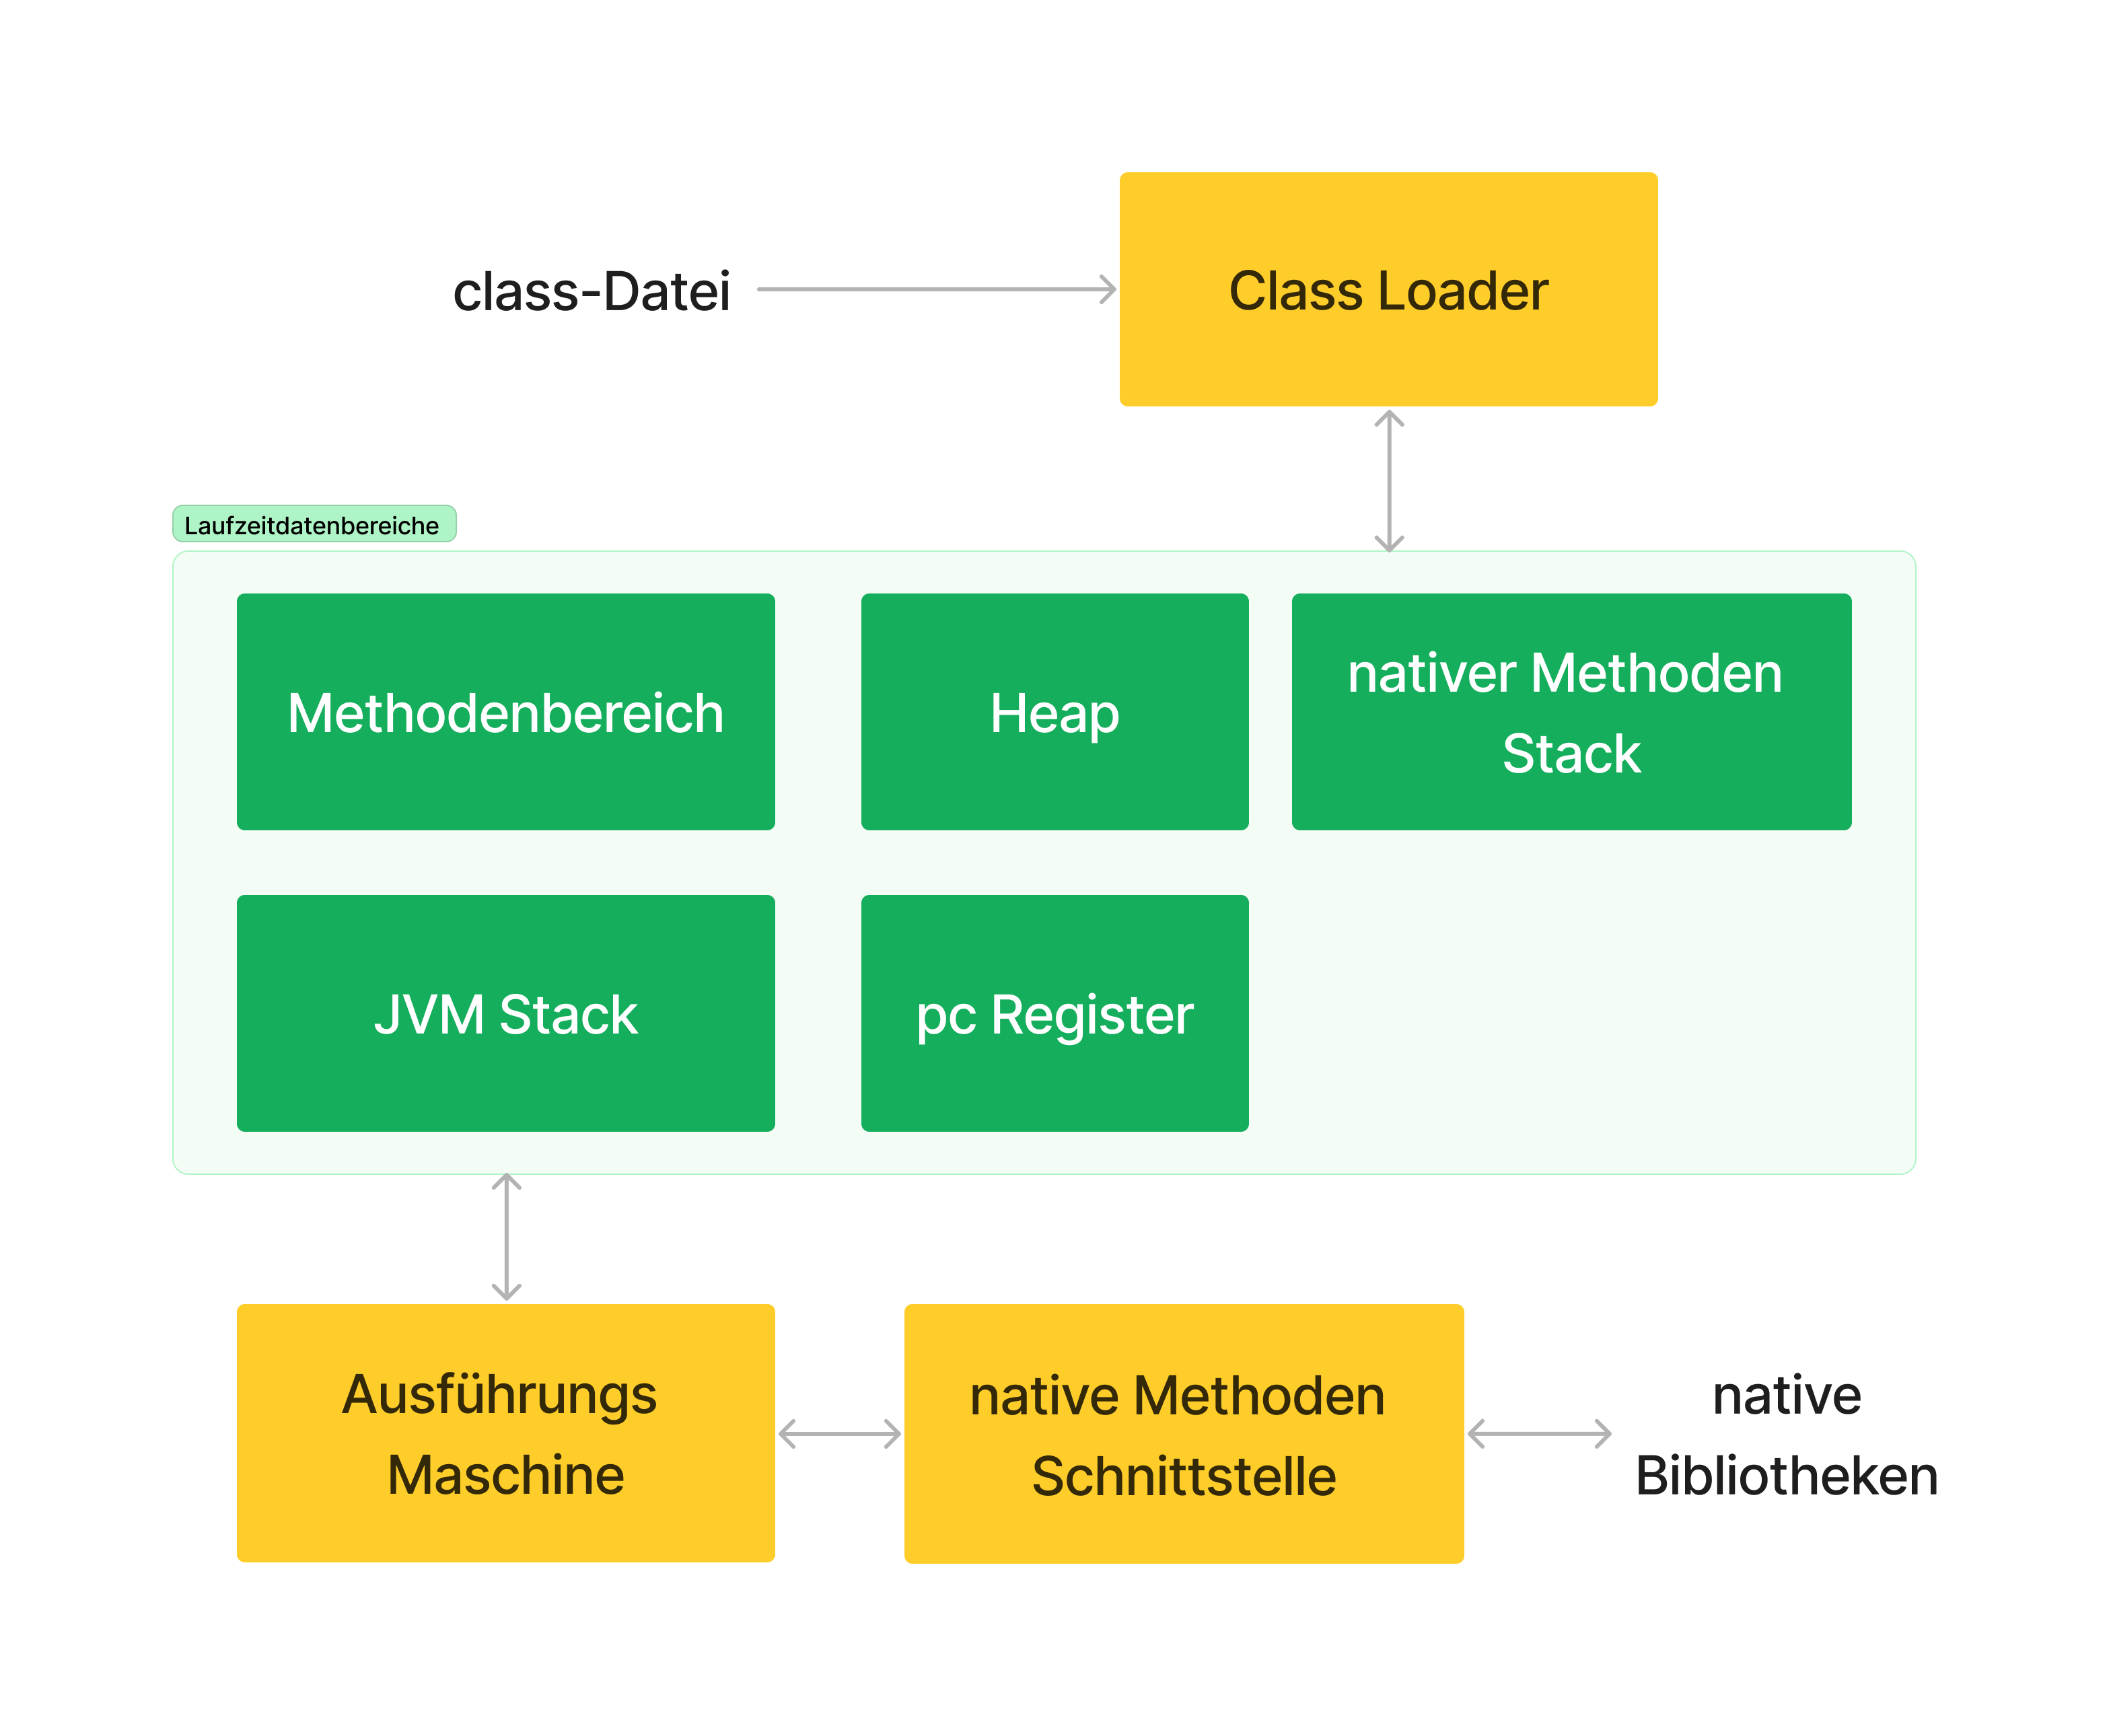
\includegraphics[width=\textwidth]{JVM.Architecture}
    \label{fig:jvm-architecture}
\end{figure}

\section{Bytecode}

Da die JVM nicht direkt den Code von JVM-basierten Programmiersprachen lesen kann, benötigt es eine Zwischensprache, den Bytecode. Dieser Bytecode entsteht bei der Übersetzung von JVM-basierten Programmiersprachen. Die class-Dateien, die bei der Übersetzung des Quelltextes erzeugt werden, enthalten als Resultat diesen Bytecode innerhalb der Methodenrümpfe.

Eine Anweisung des Bytecodes besteht aus einem Opcode, auch \textit{mnemonic} genannt, gefolgt von keinem oder mehr Operanden. Oft folgen dem Opcode keine Operanden.~\autoref{lst:jvm_bytecodeloop} zeigt die illustrative Schleife, die den Bytecode interpretiert, \parencite[siehe S. 25]{lindholm2016java}.

\begin{JavaCode}[numbers=none, caption={Auszug aus der JVM Spezifikation, welche die Interpretationsschleife für Bytecode repräsentiert.}, label=lst:jvm_bytecodeloop]
do {
    atomically calculate pc and fetch opcode at pc;
    if (operands) fetch operands;
    execute the action for the opcode;
} while (there is more to do);
\end{JavaCode}

Opcodes sind für die verschiedenen Typen der JVM separat implementiert. Will die Entwickler:in zum Beispiel zwei Variablen vom Typ \texttt{int} und \texttt{double} laden, um diese später zu addieren, müssen diese im ersten Schritt mit den beiden Opcodes \texttt{iload} und \texttt{dload} geladen werden. Nach dem Laden der beiden Werte liegen diese nun am Operanden-Stack.

Einige Opcodes, \texttt{iload} unter anderem, haben zusätzliche Varianten, die einen Suffix im Format \texttt{\_<number>} enthalten. Das Verhalten dieser Opcodes unterscheidet sich nicht von den suffixlosen Varianten, sondern dient als Speicherplatzsparmaßnahme. Die Zahl am Ende des Suffixes stellt den Index im lokalen Variablenfeld dar, auf das der Opcode zugreift. Dadurch vermeidet die JVM die Notwendigkeit eines zusätzlichen Parameters für häufig verwendete Indizes und spart ein Byte Speicherplatz.  Die Anzahl an Varianten ist je nach Opcode unterschiedlich. \texttt{iload} bietet zum Beispiel \texttt{iload\_0} bis \texttt{iload\_3}. 

Da es sich bei den Operanden der Addition um zwei verschiedene Typen handelt, konvertiert man den kleineren Typ (in diesem Fall \texttt{int}) zum größeren Typ mit dem Opcode \texttt{i2d}. Vom Namen lässt sich ableiten, dass diese Anweisung die Ganzzahl zu einer Gleitkommazahl konvertiert. Wichtig hierbei ist, dass der zu konvertierende Wert oben am Operanden-Stack aufliegen muss, da die Operation \texttt{i2d} den obersten Wert des Operanden-Stack entnimmt und den konvertierten Wert anschließend zurücklegt.

Mit zwei Gleitkommawerten kann man nun anschließend \texttt{dadd} aufrufen. Diese Operation entnimmt die beiden obersten Werte dem Operanden-Stack, errechnet die Summe und legt diese anschließend wieder auf den Operanden-Stack.

All diese Operationen sind für alle weiteren Typen der JVM definiert und sind der Spezifikation zu entnehmen. Die Größe aller Opcodes ist zugunsten der Kompaktheit auf ein Byte beschränkt. Daraus ergibt sich eine maximale Anzahl von 256 Opcodes.
\chapter{Generierung des Bytecodes mit ASM}
\label{cha:asm}
\chapter{Implementierung}
\label{cha:implementation}

Die Implementierung des Compilers ist in zwei Teile aufgeteilt: Frontend und Backend. Die Kommunikation zwischen den beiden Teilen erfolgt mithilfe eines abstrakten Syntaxbaums (AST - \textit{abstract syntax tree}), welchen das Frontend erzeugt. Dieses Kapitel geht  auf die Architektur und Implementierung dieser Teile ein.~\autoref{fig:compiler-architecture} zeigt die Archtektur des \toya Compilers. Auf die genauere Implementierung der verschiedenen Schritte des Compilers geht dieses Kapitel ein.

Die Implementierung erfolgt in Kotlin, was das Einbinden von bereits existierenden Bibliotheken des JVM Ökosystems problemlos ermöglicht. Konkret geht es dabei um ANTLR und ObjectWeb ASM, welche wichtige Rollen im Compiler übernehmen. Die Möglichkeit, Summentypen in Form von \textit{sealed} Schnittstellen und Klassen implementieren zu können, erleichert die Abarbeitung des AST wesentlich.

\begin{figure}[h]
    \caption{Compiler-Architektur}
    \centering
    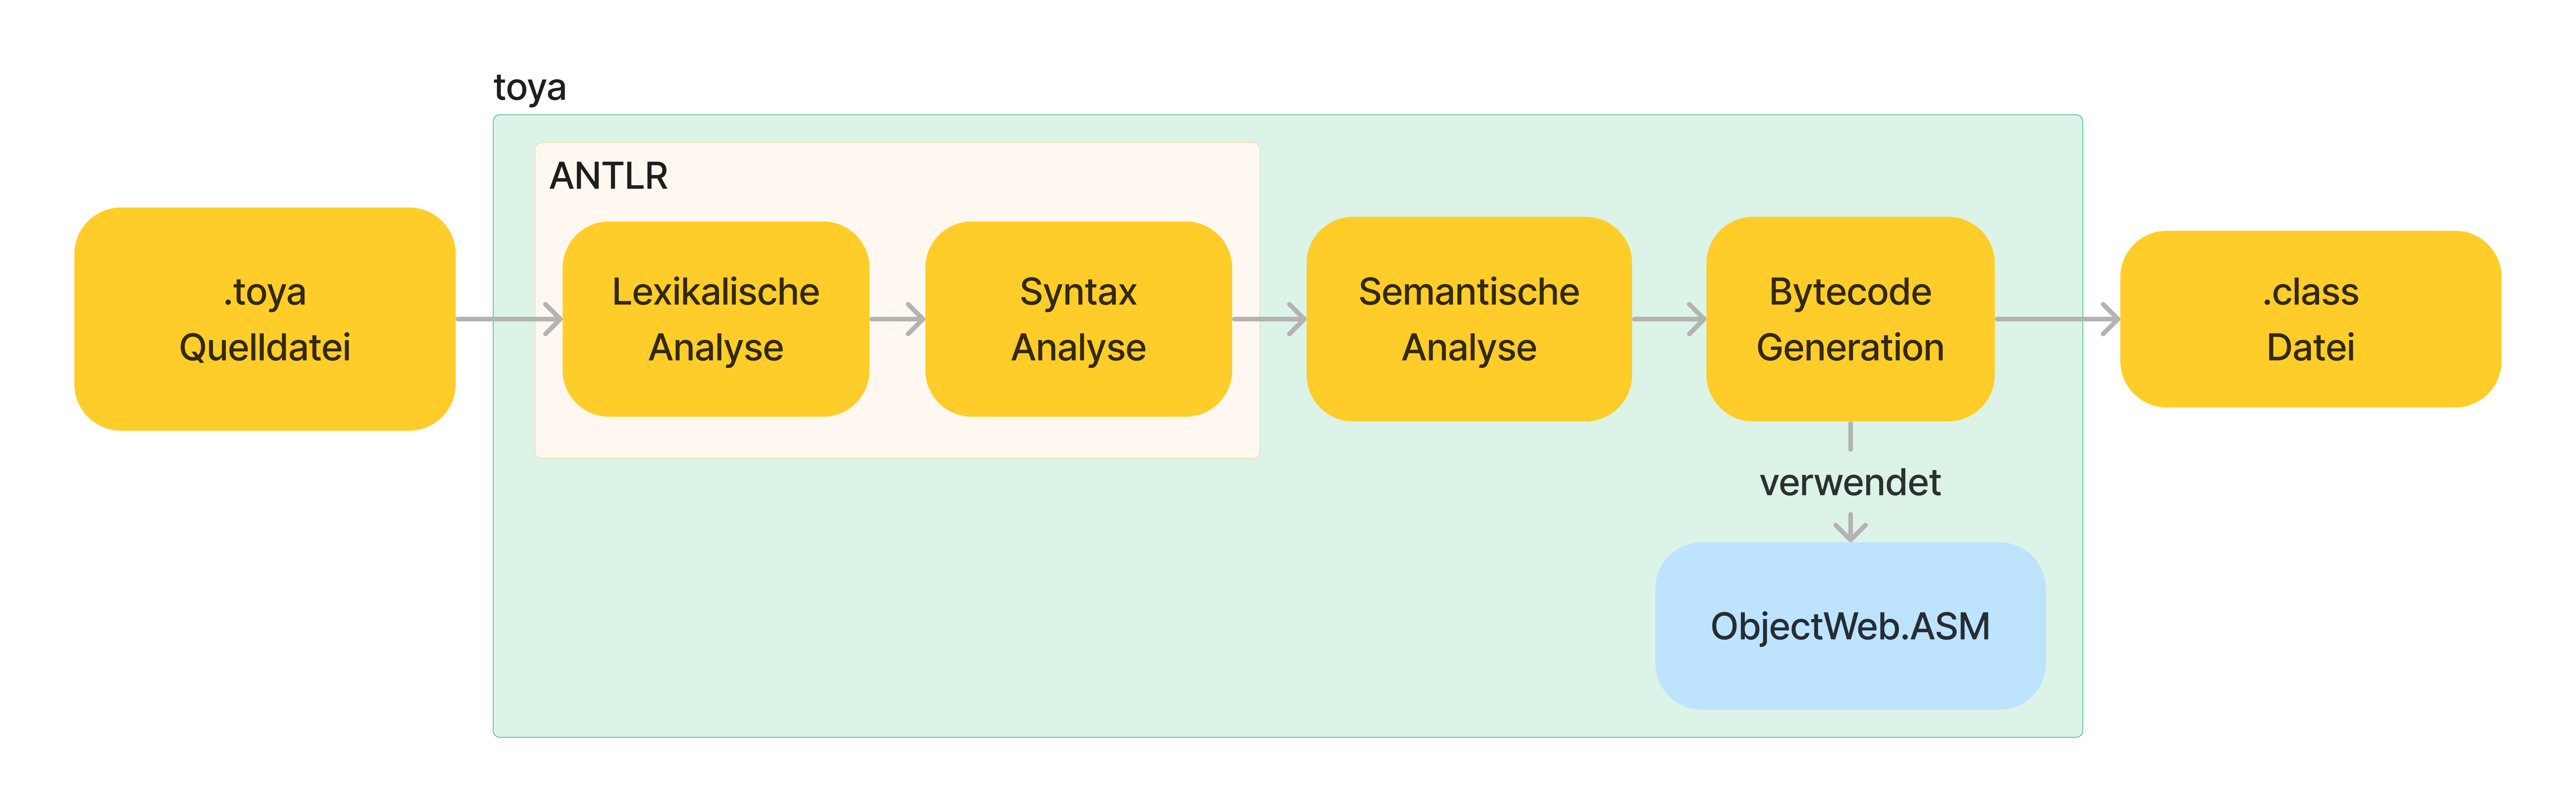
\includegraphics[width=\textwidth]{Compiler.Architecture}
    \label{fig:compiler-architecture}
\end{figure}

\section{Frontend}

Im Frontend erfolgt die lexikalische, syntaktische und teilweise die semantische Analyse. Die lexikalische Analyse zerlegt anhand der bereitgestellten Grammatik den Quellcode in \token. Anhand dieser \token erstellt die syntaktische Analyse den Syntaxbaum, welcher als Basis für den abstrakten Syntaxbaum dient.

\subsection{Grammatik}

Als Ausgangspunkt des Frontends dient die Grammatik, anhand welcher ANTLR die lexikalische und syntaktische Analyse implementiert. Diese Grammatik definiert die Compiler-Bauer:in in einer \texttt{g4}-Datei. Leerzeichen haben keine semantische Relevanz, weshalb \toya diese in der syntaktischen Analyse überspringt. Als \token definiert \toya folgende Zeichen:

\begin{itemize}
    \item Die Schlüsselwörter \texttt{match}, \texttt{for}, \texttt{for}, \texttt{if}, \texttt{else}, \texttt{var}, \texttt{true}, \texttt{false} und \texttt{null}
    \item Die Infix-Operatoren \texttt{>}, \texttt{>=}, \texttt{<}, \texttt{<=}, \texttt{==}, \texttt{!=}, \texttt{\&\&}, \texttt{||} und der Präfix-Operator \texttt{!}
    \item Die arithmetischen Operatoren \texttt{+}, \texttt{-}, \texttt{*} und \texttt{/}
\end{itemize}

Beim Versuch, ein Schlüsselwort als Variablenname zu Verwenden tritt der Ausnahmezustand \texttt{VariableNameIsKeywordException} ein. 

\subsection{Abarbeitung des Syntaxbaumes}

Wie bereits in \nameref{cha:antlr} erläutert, bietet ANTLR die Entwurfsmuster \visitor und \listener an, um den Syntaxbaum zu traversieren. \Toya verwendet das \visitor-Muster aufgrund des Umfangs des abzuarbeitenden Syntaxbaumes. Das Resultat des \visitors ist ein AST mit dem Wurzelelement \texttt{Compilation}. Diese Klasse speichert die Funktionssignaturen und ein globales \scope, welches sich über das ganze Programm erstreckt. Alle weiteren \texttt{Scopes} nehmen dieses globale \scope als Grundlage. 

Die wichtigste Methode des \visitors, welche die Abarbeitung des Syntaxbaumes überhaupt ermöglicht ist die \texttt{accept} Methode. Diese Methode benötigt als Parameter einen \visitor vom generischen Typ \texttt{ParseTreeVisitor}. \Toya implementiert folgende \visitors:

\begin{itemize}
    \item CompilationVisitor
    \item StatementVisitor
    \item BranchVisitor
    \item CompositeVisitor
    \item ExpressionVisitor
    \item FunctionSignatureVisitor
    \item FunctionVisitor
\end{itemize}

Um das Traversieren der Knoten des Syntaxbaumes zu ermöglichen, generiert ANTLR für alle Regeln der Grammatik-Definition Methoden im Format \texttt{visit<RuleName>(ctx: toyaParser.<RuleName>Context)}. Jede dieser Methoden liefert einen Wert vom generischen Typ \texttt{toyaBaseVisitor} zurück.~\autoref{lst:impl_visitor} zeigt die \texttt{visit}-Funktion für Variablendeklarationen.

\begin{KotlinCode}[numbers=none, caption={\visitor-Funktion zum Erstellen eines \texttt{VariableDeclarationStatement}}, label=lst:impl_visitor]
class StatementVisitor(val scope: Scope) : toyaBaseVisitor<Statement>() {
    override fun visitVariableDeclaration(ctx: toyaParser.VariableDeclarationContext): Statement {
        val varName = ctx.name().text
        if(varName.isReservedKeyword()) throw VariableNameIsKeywordException(varName)
        val expression = ctx.expression().accept(ExpressionVisitor(scope))
        scope.addLocalVariable(LocalVariable(varName, expression.type))
        return VariableDeclarationStatement(varName, expression)
    }
    // Rest of class
}
\end{KotlinCode}

Zur Behandlung von Syntaxfehler bietet ANTLR die Klasse \texttt{BaseErrorListener} um der Benutzer:in relevante Informationen anzuzeigen. \Toya zeigt mithilfe dieser Klasse an, welche Anweisung in welcher Zeile und welches Zeichen die syntaktische Analyse verhindert.

\subsection{Typ-System}

Die Basis für das Typ-System in \toya ist die Schnittstelle \texttt{Type} und die davon abgeleitete Enum-Klasse \texttt{BasicType}, welche alle in \toya verfügbaren Typen beinhaltet. \Toya erlaubt keine explizite Definition des Typs einer Variable, weshalb der Typ immer vom Wert der Variable abzuleiten ist. Den Typ einer Variable ermittelt \toya mithilfe der Klasse \texttt{TypeResolver}. Anhand von regulären Ausdrücken ermittelt die Funktion \texttt{getFromValue} den Typ des Wert-Literals, wie in~\autoref{lst:impl_getvalue} zu sehen ist.

\begin{KotlinCode}[numbers=none, caption={Methode zur Ermittlung des Typs bei Wert-Literalen}, label={lst:getFromValue}, label=lst:impl_getvalue]
fun getFromValue(value: String?): Type {
    if (value.isNullOrEmpty()) return BasicType.VOID
    if (isBoolean(value)) return BasicType.BOOLEAN
    if (isDouble(value)) return BasicType.DOUBLE
    if (isInt(value)) return BasicType.INT
    if (isString(value)) return BasicType.STRING
    throw UnableToInferTypeException(value)
}
\end{KotlinCode}

Da nun jeder Ausdruck Typinformationen besitzt, ermöglicht das die semantische Analyse von Ausdrücken. Die Erweiterungsfunktion \texttt{Type.checkTypeMatch} überprüft, ob beide Operanden vom selben Typ sind. Wenn nicht, kommt es zu einem Ausnahmezustand. Die Implementierung für \texttt{Type.checkTypeMatch} ist in~\autoref{lst:impl_checktypematch} zu sehen.

\begin{KotlinCode}[numbers=none, caption={Methode zur Überprüfung von übereinstimmende Typen zweier Operanden}, label=lst:impl_checktypematch]
fun Type.checkTypeMatch(rhs: Type) {
    if (this != rhs) throw BinaryOperationTypeMismatchException(this, rhs)
}    
\end{KotlinCode}

\subsection{Standardfunktionen}

Standardfunktionen sind Funktionen, welche jedem \toya-Programm ohne Weiteres zur Verfügung stehen. Standardfunktionen sind kein Bestandteil der lexikalischen Analyse. Die Funktion \texttt{visitFunctionCall} des \texttt{ExpressionVisitors} prüft mithilfe der Funktion \texttt{isStandardFunction}, ob es sich bei einer Funktion um eine Standardfunktion handelt. Ist dies der Fall, erzeugt der \visitor kein Objekt vom Typ \texttt{FunctionCall}, sondern ein Objekt, welches von \texttt{StandardFunction} erbt. Im Falle der Funktion \texttt{print} ist das zum Beispiel \texttt{PrintFunction}.

Standardmäßig bietet \toya die Standardfunktion \texttt{print} an, welche einen Aufruf der Java Funktion \texttt{System.out.println} durchführt. Die Architektur des \toya Compilers ist darauf ausgelegt weitere Standardfunktionen hinzufügen zu können. Besteht dieser Wunsch, sind an folgenden Stellen von Entwicklerseite her Veränderungen vorzunehmen:

\begin{itemize}
    \item Im \texttt{when} innerhalb der \texttt{ExpressionVisitor.visitFunctionCall} Funktion muss ein Fall für die zu implementierenden Funktion hinzugefügt werden.
    \item Innerhalb der \texttt{StandardFunctions.kt} Datei: In der \texttt{standardFunctions} Liste ist eine FunktionsSignatur der neuen Standardfunktion hinzuzufügen und eine Klasse, welche \texttt{StandardFunction} implementiert und von und \texttt{Expression} erbt, zu definieren.
    \item In der \texttt{StandardFunctionGenerator} Klasse ist der Code zum Generieren des Bytecodes zu definieren.
\end{itemize}

\section{Abstrakter Syntaxbaum}

Die explizite Umwandlung auf einen abstrakten Syntaxbaum ist theoretisch nicht immer nötig. \Toya verwendet aber ANTLR und der daraus resultierende Syntaxbaum enthält teilweise zu viele Informationen. Teilweise fehlen auch notwendige Informationen, wie zum Beispiel Typinformationen eines Ausdrucks. Daher macht es Sinn, diesen Syntaxbaum auf einen AST umzubauen.

Ein Großteil des AST behandelt die Einteilung von Ausdrücken und Anweisungen in ein granulareres Klassen-Schema. Die Einteilung in zum Beispiel \texttt{LessEqualExpression} und \texttt{ForStatement} anstatt die bloße Gliederung in \texttt{Expression} und \texttt{Statement} ermöglicht eine gut skalierbare und nachvollziehbare Lösung für die Bytecode-Generierung im Backend. Die Klassenhierarchie für \texttt{Statement} und \texttt{Expression} ist in~\autoref{fig:ast-architecture} zu sehen. Schnittstellen sind grün markiert, abstrakte Klassen orange.

\begin{figure}[h]
    \caption{AST-Architektur für Ausdrücke und Anweisungen.}
    \centering
    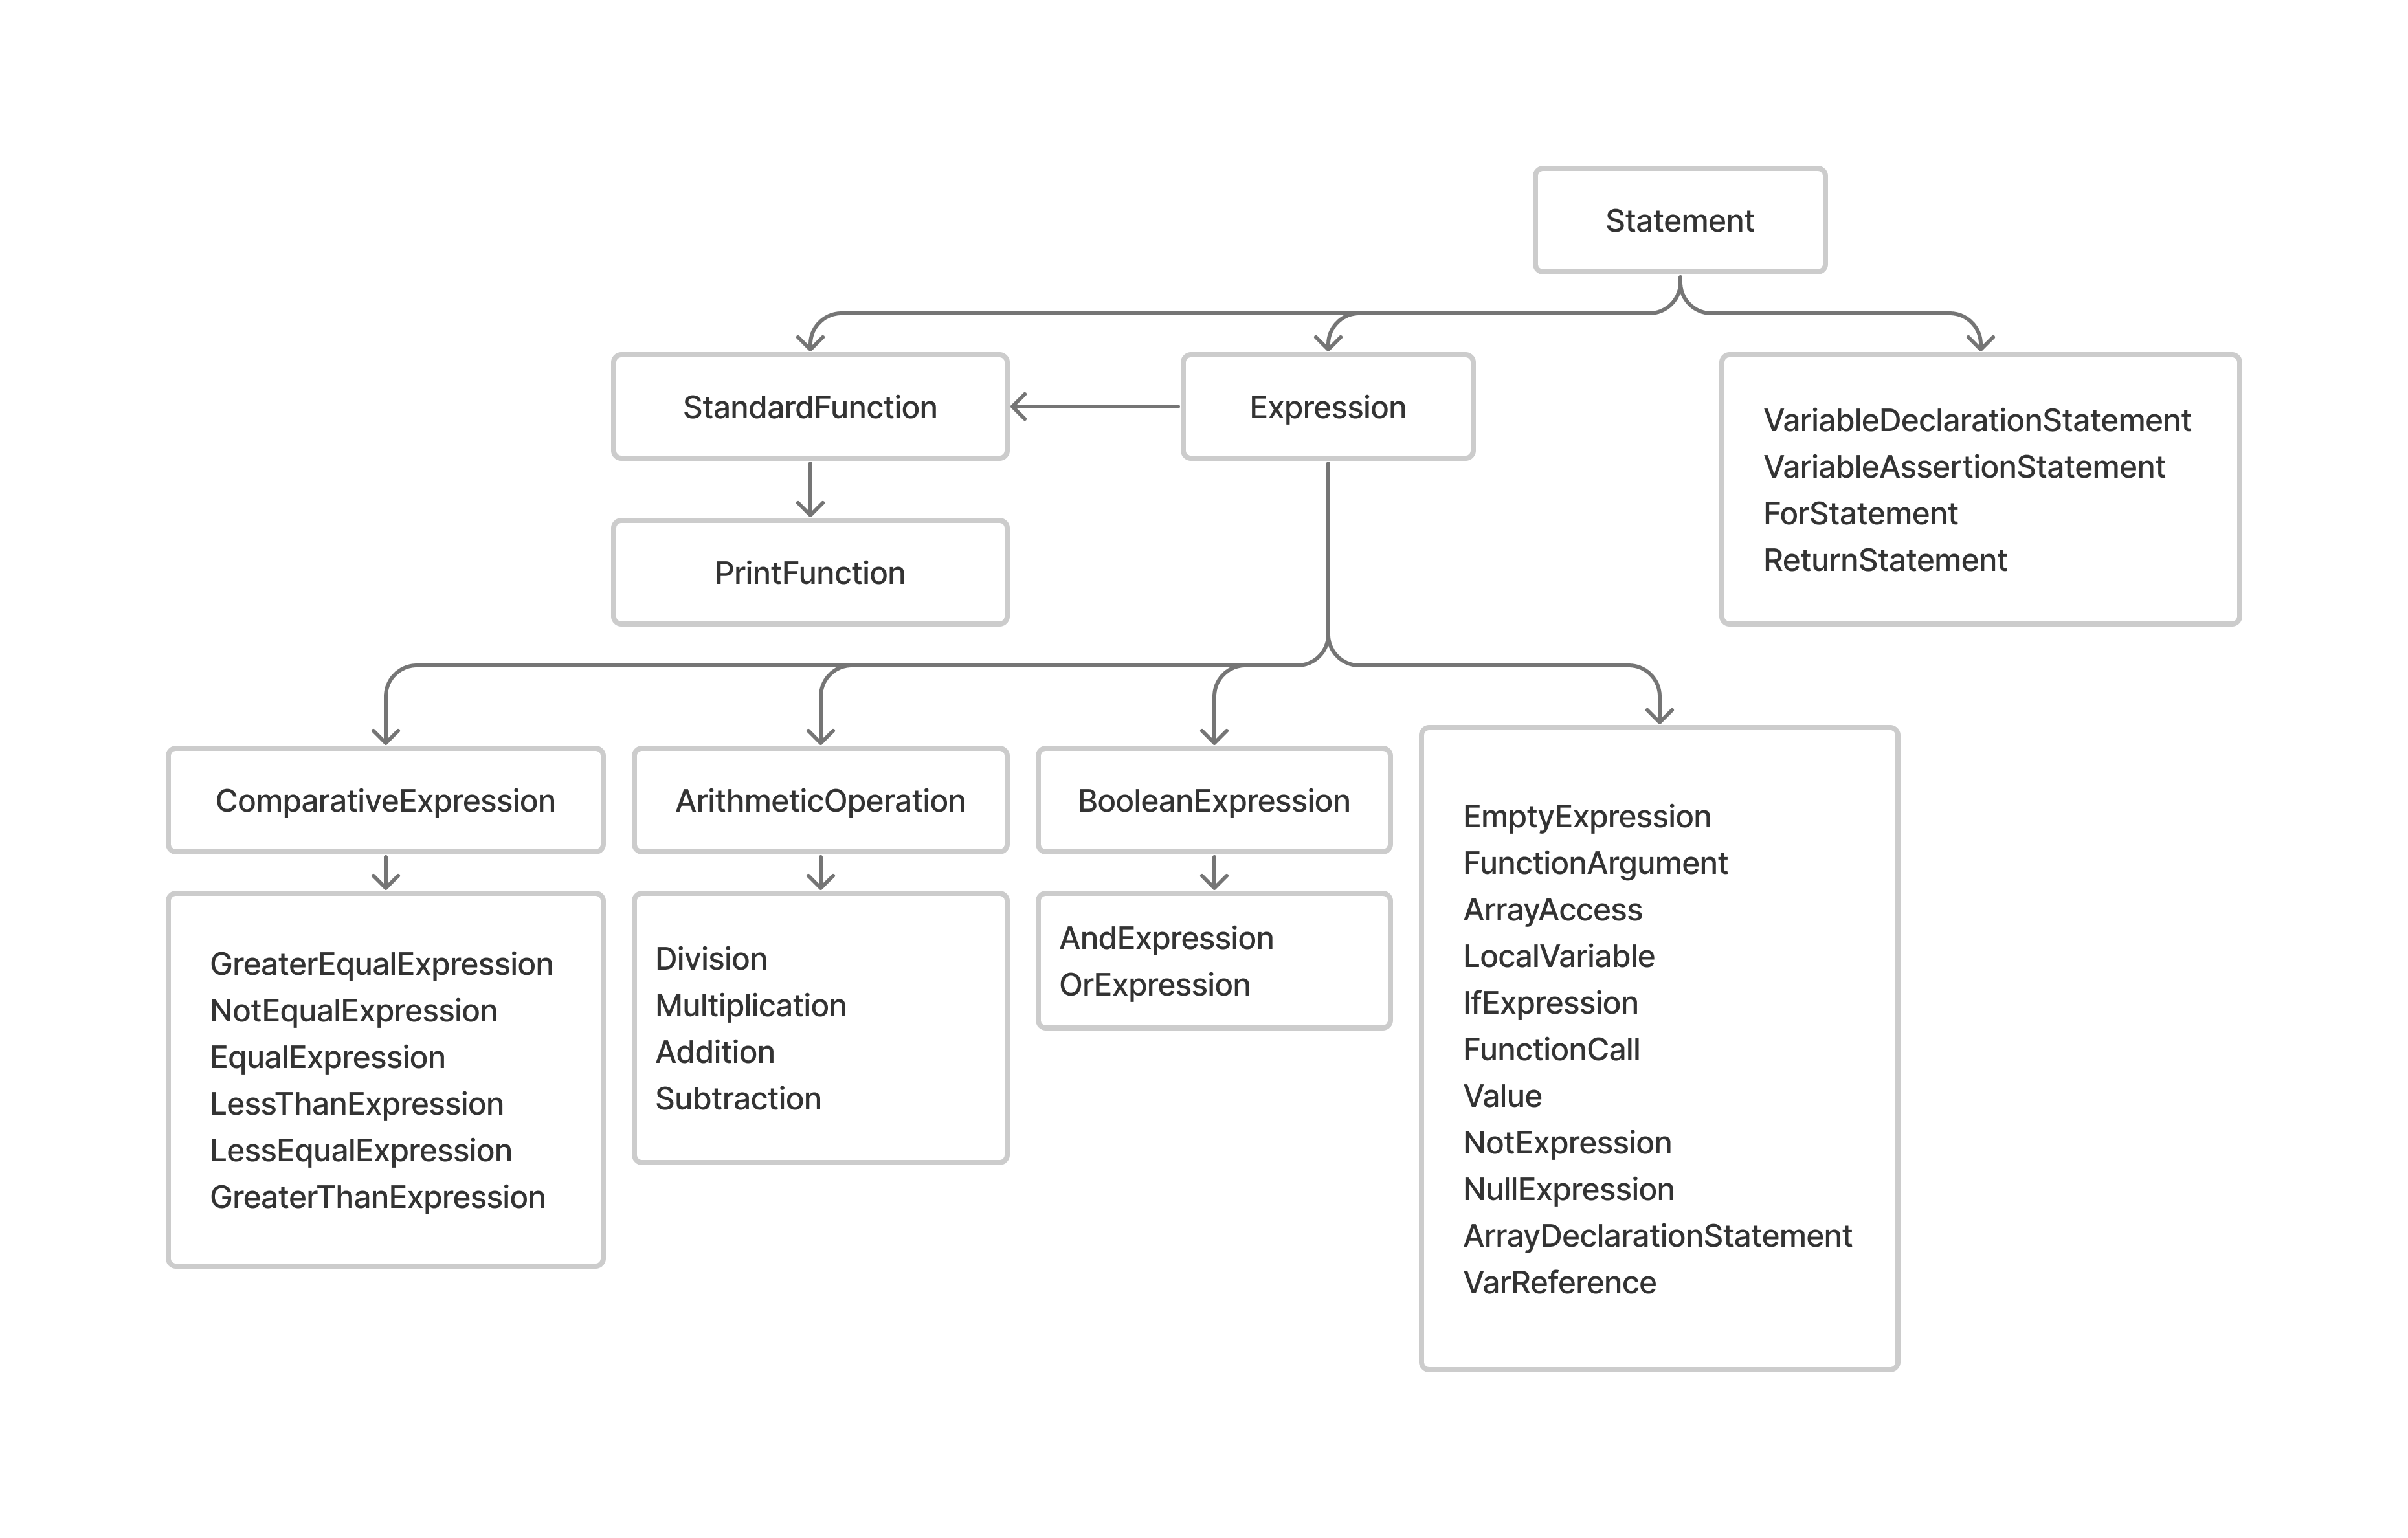
\includegraphics[scale=0.2]{AST.Diagram}
    \label{fig:ast-architecture}
\end{figure}

Kotlin bietet zur kompakten Erstellung von Datenobjekten sogenannte \textit{data classes} an. \texttt{data class} Objekte erzeugen für Parameter des primären Konstruktors folgende Funktionen:

\begin{itemize}
    \item \texttt{equals} und \texttt{hashCode}.
    \item \texttt{toString} im Format \texttt{Addition(left=42, right=31)}.
    \item \texttt{component<1-n>}, die bei der Destrukturierung von Objekten verwendet werden. Hierbei ist die Reihenfolge der Definition relevant.
    \item \texttt{copy} zum durchführen einer tiefen Kopie des Objekte.
\end{itemize}

\Toya verwendet \textit{data classes} für fast alle Klassen des AST. Ausgenommen davon sind Basisklassen, von denen andere Klassen ableiten, da die Vererbung einer \textit{data class} zu Problemen mit dem Verhalten der \texttt{equals} Funktion führt. Java bietet seit Version 14 das Schlüsselwort \texttt{record} als Äquivalent zu diesem Konzept an. Jedoch fehlen bei \texttt{record} die \texttt{copmonentN} und \texttt{copy} Funktionen.

Die \texttt{Scope} Klasse ist eine zentrale Komponente zur Verwaltung des AST und wird unter anderem für die semantische Analyse benötigt. Sie speichert die lokalen Variablen für einen gegebenen Block und die Methodensignaturen eines \toya Programms. Bei Operationen, deren Operanden lokale Variablen sind, überprüft \toya mithilfe von \texttt{Scope}, ob diese Variablen im momentanten Kontext zur Verfügung stehen.

Im Zuge der Bytecode-Generierung ermittelt \toya mithilfe \scope den Index einer lokalen Variable. Hierbei reicht es nicht aus, den Index der Variable in der Liste \texttt{localVariables} zu ermitteln. Variablen vom Typ \texttt{double} und \texttt{long} benötigen zwei Plätze im \textit{Run-Time Constant Pool}, da deren Indizes 16 Bit, anstatt der üblichen acht Bit einnehmen. Da \toya den Typ Double implementiert, ist diese Eigenschaft zu berücksichtigen. Diese Berechnung erfolgt durch eine Reduktions-Operation in der Funktion \texttt{getLocalVariableIndex}, wie in~\autoref{lst:impl_localvariable} zu sehen ist. Diese Reduktions-Operation summiert alle Indizes inklusive dem der gesuchten Variable auf. Für Ganzzahlen addiert die Operation eins, für Gleitkommazahlen zwei zum Gesamtergebnis.

\begin{KotlinCode}[numbers=none, caption={Ermittlung des Index einer Variable in einem \texttt{Scope}}, label=lst:impl_localvariable]
fun getLocalVariableIndex(varName: String) : Int {
    // hotfix for handling 2-wide index types (double, long, etc)
    return localVariables
        .subList(0, localVariables.indexOf(getLocalVariable(varName)))
        .fold(0) { acc, next ->
            acc + if (next.type == BasicType.DOUBLE) 2 else 1
        }
}
\end{KotlinCode}

\texttt{Scope} verwaltet nicht nur Variablen, sondern auch Funktionssignaturen. Beim Aufruf einer Funktion, überprüft \scope, ob diese Funktion auch definiert ist. Wenn nicht, tritt der Ausnahmezustand \texttt{MethodSignatureNotFoundException} ein. Während das Überladen von Funktionen erlaubt ist, können keine Funktionen mit identischer Signatur existieren, da diese in einem \texttt{Set} gespeichert sind.

\section{Backend}

Das Backend hat als zentrale Aufgabe die Code-Generierung anhand des abstrakten Syntaxbaumes, den das Frontend erzeugt hat. Zum Erzeugen des Bytecodes verwendet das Backend ObjectWeb ASM als zentrale Bibliothek. Als Resultat liefert das Backend ein Byte-Feld, das anschließend ein \texttt{FileOutputStream} in eine class-Datei schreibt.

\subsection{ObjectWeb ASM}

ObjectWeb ASM ist eine Bibliothek zum Lesen, Bearbeiten und Erzeugen von Bytecode für die JVM. Sie bietet eine Schnittstelle, um Funktionen, Klassen und einzelne Anweisungen zu erzeugen. \Toya verwendet ASM zum Erzeugen einer Klasse und Funktionen anhand des AST. Neben der Bytecode-Generierung erfolgt im Backend der Teil der semantischen Analyse für welchen Informationen des AST notwendig sind. ASM ist kein Akronym sondern eine Anlehnung an das Schlüsselwort \texttt{asm} in der Programmiersprache C \parencite{bruneton2002asm}.

Da \toya keine Definition von Klassen erlaubt, reicht es aus, eine statische Klasse, unabhängig vom eigentlichen Quelltext zu generieren. Version dieser Klasse ist 52, was Java 8 entspricht. Einen höhere Version ist nicht nötig, da alle Bestandteile von \toya sehr primitiv sind.

Klassen erstellt ASM mithilfe des \texttt{ClassWriter}. Der Konstruktor dieser Klasse hat einen Parameter \texttt{flags}, das der \toya Compiler mit \texttt{COMPUTE\_FRAMES + COMPUTE\_MAXS} initialisiert. \texttt{COMPUTE\_MAXS} und \texttt{COMPUTE\_FRAMES} ermöglicht die automatische Berechnung der maximal erlaubten Anzahl an lokalen Variablen, die maximale Größe des Stacks und die Berechnung aller \textit{Stack Map Frames}. Siehe dazu~\autoref{lst:impl_classwriter}.

\begin{KotlinCode}[numbers=none, caption={Erstellung einer Klasse mithilfe ObjectWeb ASM}, label=lst:impl_classwriter]
val classWriter: ClassWriter = ClassWriter(
    ClassWriter.COMPUTE_FRAMES + ClassWriter.COMPUTE_MAXS
)
classWriter.visit(
    CLASS_VERSION,
    Opcodes.ACC_PUBLIC,
    className,
    null,
    "java/lang/Object",
    null
)
\end{KotlinCode}

Zum Erzeugen von Methoden und und deren Logik bietet ASM die Klasse \texttt{MethodWriter}. Diese Klasse ermöglicht das Schreiben der Bytecode Anweisungen innerhalb einer Methode. Außerdem ermöglicht \texttt{MethodWriter} unter anderem auch das Setzen von \textit{Labels} um Sprung-Befehle durchführen zu können. Sprung-Befehle sind für den Kontrollfluss wichtig, um in If-Verzweigungen nicht zutreffende Zweige zu überspringen und um bei For-Schleifen an den Beginn der Schleife zurückzukehren.~\autoref{lst:impl_generateexample} zeigt die \texttt{generate}-Funktion zum Generieren von Wertliteralen mithilfe von ObjectWeb ASM.

\begin{KotlinCode}[numbers=none, caption={\texttt{generate} Funktion, welche Wert-Literale erzeugt.}, label=lst:impl_generateexample]
private fun generate(value: Value) {
    val type = value.type
    val stringValue = value.value

    type.handleTypeGroups(
        i = {
            val intValue = stringValue.toInt()
            methodVisitor.visitLdcInsn(intValue)
        },
        d = {
            val doubleValue = stringValue.toDouble()
            methodVisitor.visitLdcInsn(doubleValue)
        },
        a = { methodVisitor.visitLdcInsn(stringValue.trim('"')) },
        z = {
            val opcode = if (stringValue == "true") Opcodes.ICONST_1 else Opcodes.ICONST_0
            methodVisitor.visitInsn(opcode)
        }
    )
}
\end{KotlinCode}

\subsection{Summentypen}

Im Backend kommen Summentypen in Form von \textit{sealed classes} zum Einsatz. \textit{Sealed classes} in Kotlin besitzen die besondere Eigenschaft, dass alle Kindklassen zur Übersetzungszeit vollständig bekannt sind. Dies ermöglicht zum Beispiel die Verwendung von erschöpfenden \texttt{when}-Ausdrücken in Kombination mit Polymorphismus. Kindklassen einer \textit{sealed class} sind alle im selben Modul zu definieren. Neben Klassen können auch Schnittstellen als \texttt{sealed} markiert sein. \textit{Selead classes} sind zusätzlich implizit eine abstrakte Klasse.

Wichtige \textit{sealed classes} und \textit{sealed interfaces} des abstrakten Syntaxbaums sind folgende:

\begin{itemize}
    \item \texttt{ArithmeticOperation}: Umfasst Ausdrücke Addition, Subtraktion, Multiplikation und Division.
    \item \texttt{BooleanExpression}: Umfasst Ausdrücke für die logischen Operatoren Und und Oder. Eine \texttt{BooleanExpression} liefert immer einen boole'schen Wert zurück.
    \item \texttt{ComparativeExpression}: Umfasst Ausdrücke für Größer, Größer-Gleich, Gleich, Kleiner, Kleiner-Gleich und Ungleich. Eine \texttt{ComparativeExpression} liefert immer einen boole'schen Wert zurück.
    \item \texttt{Branch}: Umfasst die beiden Möglichkeiten, Verzweigungen im Kontrollfluss entweder als Anweisungsblock oder als einzelnen Ausdruck zu definieren.
\end{itemize}

\subsection{Architektur der Code-Generierung}

Der Ablauf der Code-Generierung ist auf fünf Klassen aufgeteilt, wie in~\autoref{fig:backend-flowchart} zu sehen ist. Als Einstiegspunkt dient immer die Klasse \texttt{ByteCodeGenerator}. Diese Klasse erzeugt eine öffentliche Klasse, die von \texttt{Object} erbt. Als nächstes ruft die Klasse \texttt{ByteCodeGenerator} die \texttt{generate}-Methode der Klasse \texttt{FunctionGenerator} für jede Funktion des \toya Programmes auf.

Der \texttt{FunctionGenerator} iteriert über die Liste aller Anweisungen der Funktion und ruft für jede Anweisung die \texttt{generate}-Funktion des \texttt{StatementGenerator auf}. Nach dem durchlaufen der Anweisungsliste überprüft der \texttt{FunctionGenerator}, ob die Funktion als letzte Anweisung eine Rückgabeanweisung definiert und ob die Funktion überhaupt einen Wert zurückliefert. Liefert die Funktion einen Wert zurück, hat aber keine Rückgabeanweisung an letzter Stelle, muss der Compiler diese Anweisung generieren. Anhand des Typs der letzten Anweisung der Funktion wählt der \texttt{FunctionGenerator} nun den richtigen Opcode aus und generiert die Anweisung mithilfe von ObjectWeb ASM. Ist die letzte Anweisung zum Beispiel ein Ausdruck vom Typ \texttt{int}, generiert der \toya Compiler den Opcode \texttt{ireturn}.

Der \texttt{StatementGenerator} generiert entweder eine Anweisung selbst oder delegiert diese Aufgabe an den \texttt{ExpressionGenerator}, wenn es sich bei der Anweisung um einen Ausdruck handelt. Konkret generiert der \texttt{StatementGenerator} Bytecode für Variablen- und Felddeklarationen, Variablenzuweisungen, explizite Rückgabeanweisungen und For-Schleifen. Ein Großteil der Komplexität in dieser Klasse stammt daher, dass verschiedene Opcode für die verschiedenen Typen von \toya zu beachten sind.

\begin{figure}[h]
    \caption{Ablauf der Code-Generierung im Backend.}
    \centering
    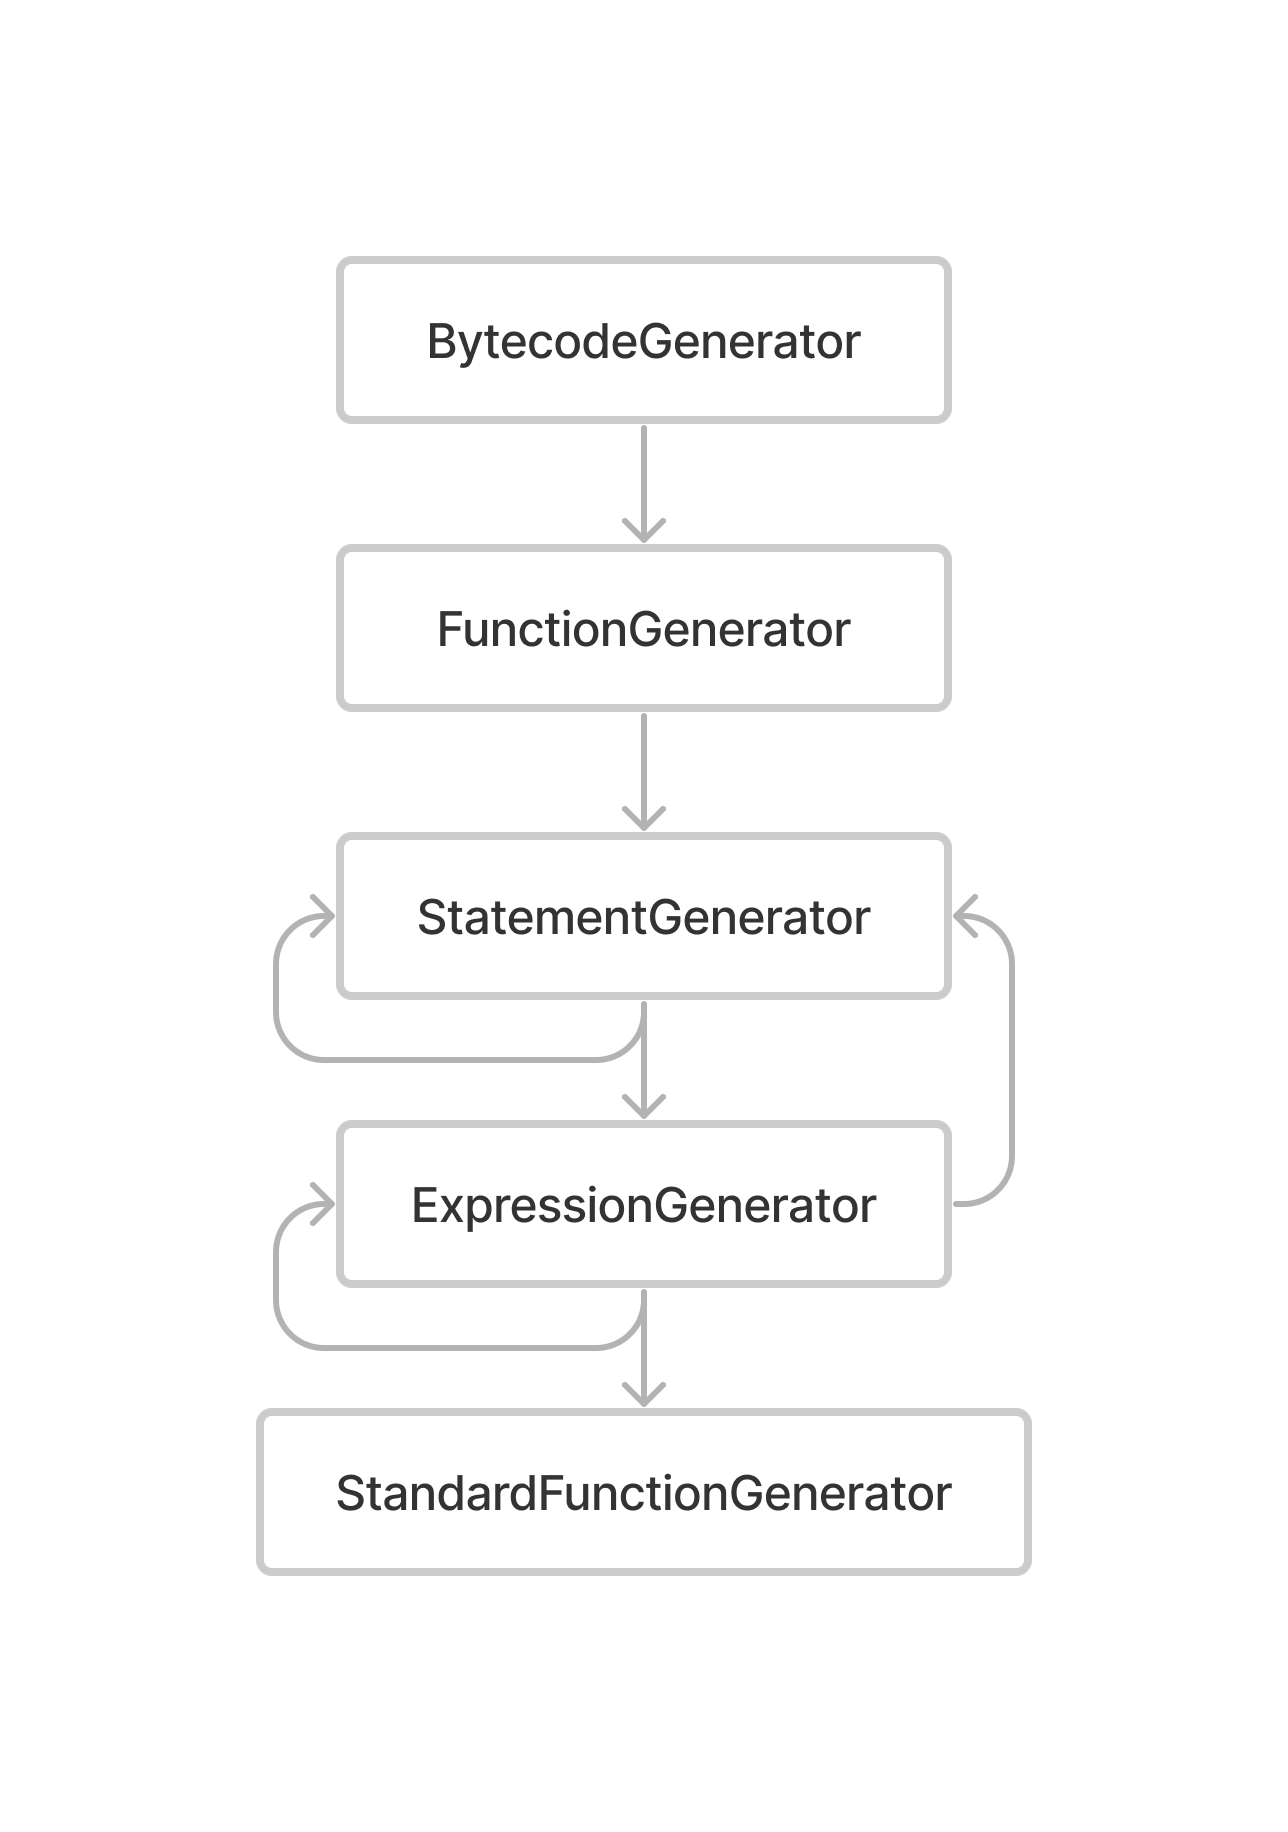
\includegraphics[scale=0.3]{Backend.Flowchart}
    \label{fig:backend-flowchart}
\end{figure}

Um den Mehraufwand für die Berücksichtigung jedes Typs so gut wie möglich zu minimieren, sind die Erweiterungsfunktionen \texttt{Type.handleTypeGroup} und\break \texttt{Type.handleTypeArrays} definiert, die Implementierung und Verwendung von letzteres ist in~\autoref{lst:impl_handletypearrays} zu sehen. Diese beiden Funktionen höherer Ordnung benötigen eine Funktion für jeden Typ als Parameter. Dadurch liegt in jeder Funktion nur der Code, der für den entsprechenden Typ relevant ist.

Ebenso ist auch die Ausnahmebehandlung mithilfe dieser Funktionen umsetzbar. Versucht man zum Beispiel zwei Referenzen oder boole'sche Ausdrücke zu addieren, tritt der Ausnahmezustand \texttt{UnsupportedOperationOnTypeException} ein. Dadurch, dass das Verhalten für jeden Typ verpflichtend definiert sein muss, vermeidet die Entwickler:in auch, dass das Verhalten für einen Typ ungeklärt bleibt.

\begin{KotlinCode}[numbers=none, caption={Die Erweiterungsfunktion \texttt{Type.handleTypeArrays}, um den richtigen Opcode zum Speichern einer Variable zu ermitteln.}, label=lst:impl_handletypearrays]
fun <T> Type.handleTypeArrays(
    ia: () -> T,
    da: () -> T,
    aa: () -> T,
    ba: () -> T
): T {
    return when (this) {
        BasicType.INT_ARR -> ia()
        BasicType.DOUBLE_ARR -> da()
        BasicType.STRING_ARR -> aa()
        BasicType.BOOLEAN_ARR -> ba()
        else -> throw NotImplementedError("handling for type '\${this.typeName}' not implemented")
    }
}

val opcode = localVariable.type.handleTypeArrays(
    ia = { Opcodes.IASTORE },
    da = { Opcodes.DASTORE },
    aa = { Opcodes.AASTORE },
    ba = { Opcodes.BASTORE }
)
\end{KotlinCode}

Der \texttt{ExpressionGenerator} generiert Ausdrücke oder delegiert Standardfunktionsaufrufe an den \texttt{StandardFunctionGenerator}. Ist der konkrete Typ des Ausdrucks \texttt{PrintFunction}, delegiert der \texttt{ExpressionGenerator} die Bytecode-Generierung an den \texttt{StandardFunctionGenerator}. Konkret generiert der \texttt{ExpressionGenerator} Bytecode für folgende Ausdrücke:

\begin{itemize}
    \item Variablenaufrufe
    \item Funktionsaufrufe
    \item Funktionsargumente
    \item Wertliterale
    \item arithmetische Operationen
    \item Vergleichsoperationen
    \item Logikoperationen
    \item Null-Ausdrücke
    \item Zugriff auf Felder
    \item If-Ausdrücke
\end{itemize}

Der \texttt{StandardFunctionGenerator} generiert alle Standardfunktionen. Im Falle der \texttt{PrintFunction} verwendet \toya die \texttt{System.out.println} Implementierung von Java. In einem ersten Schritt ermittelt \toya die Referenz des \texttt{PrintSteam} Typs in Form der statischen Variable \texttt{out} und evaluiert den auszugebenden Wert des Ausdrucks. Anschließend wird die \texttt{println} Funktion des \texttt{out} Objekts aufgerufen. Die \texttt{println} Funktion verwendet den oben aufliegenden Wert am Operanden-Stack, weswegen dieser Wert im ersten Schritt bereits evaluiert wurde. Die konkrete Implementierung, wie in~\autoref{lst:impl_println} zu sehen ist, wurde \textcite{enkelTutorial} entnommen.

\begin{KotlinCode}[numbers=none, caption={Bytecode zum Aufruf der \texttt{println} Funktion von Java},label=lst:impl_println]
private fun generate(printFunction: PrintFunction, scope: Scope) {
    val expression = printFunction.message
    mv.visitFieldInsn(Opcodes.GETSTATIC, "java/lang/System", "out", "Ljava/io/PrintStream;")
    expressionGenerator.generate(expression, scope)
    val type = expression.type
    val descriptor = "(\${type.getDescriptor()})V"
    val fieldDescriptor = "java/io/PrintStream"
    mv.visitMethodInsn(Opcodes.INVOKEVIRTUAL, fieldDescriptor, "println", descriptor, false)
}
\end{KotlinCode}
\chapter{Tests}
\label{cha:tests}

Um die Funktionalität von \toya zu gewährleisten, sind Tests zu vollziehen. Diese Tests umfassen die folgenden drei Schritte:
\begin{enumerate}
    \item Programmcode in \toya schreiben
    \item Den übersetzten Bytecode analysieren
    \item Die Ausgabe des Programms überprüfen
\end{enumerate}

Die Analyse des Bytecode erfolgt mit dem, in der JDK inkludierten Werkzeug \texttt{javap}. Dieses erlaubt es, den Bytecode einer class-Datei in einer für Menschen leserlichen Form auszugeben. Der Aufruf erfolgt über die Kommandozeile im Format: \texttt{javap -c Main.class}. Der Parameter \texttt{-c} zeigt zusätzlich die Bytecode Befehle innerhalb der Methoden an. Die Ausführung der Programme erfolgt über die Kommandozeile mit dem Befehl \texttt{java Main}. Insgesamt gilt es, die einzelnen Sprachkonstrukte und anschließend ein umfangreicheres Programm zu testen.

\section{Hello World}

Der erste Test stellt ein \textit{Hello World} Programm dar, wie in~\autoref{lst:test_1_source} zu sehen ist. Der Bytecode dieses Programms beschränkt sich auf einige wenige Befehle.~\autoref{lst:test_1_bytecode} zeigt den Bytecode. Konkret laden \texttt{getstatic} und \texttt{ldc} Referenzen zum \texttt{System.out} Objekt und der auszugebenden Zeichenkette. Anschließend ruft \texttt{invokevirtual} die \texttt{println} Funktion mit der Zeichenkette auf. Als Resultat gibt dieser Test die Zeichenkette \textit{Hello World} auf der Konsole aus, zu sehen in~\autoref{lst:test_1_output}.

\begin{ToyaCode}[numbers=none, caption={Quelltext des Hello World Programms},label=lst:test_1_source]
function main(args: string[]) {
    print("Hello World")
}
\end{ToyaCode}

\begin{JavaCode}[numbers=none, caption={Bytecode des Hello World Programms},label=lst:test_1_bytecode]
public class Main {
    public static void main(java.lang.String[]);
        Code:
            0: getstatic     #12    // Field java/lang/System.out:Ljava/io/PrintStream;
            3: ldc           #14    // String Hello World
            5: invokevirtual #20    // Method java/io/PrintStream.println:(Ljava/lang/String;)V
            8: return
}
\end{JavaCode}

\begin{ToyaCode}[numbers=none, caption={Konsolen-Ausgabe des Hello World Programms},label=lst:test_1_output]
Hello World    
\end{ToyaCode}

\section{Funktionen}

Der zweite Test beschäftigt sich mit der Verwendung von Funktionen und dem Arbeiten mit Funktionsergebnissen.~\autoref{lst:test_2_source} zeigt den Quelltext des Programms. Als erstes ruft dieser Test die \texttt{title} Funktion auf. Diese Funktion gibt die Zeichenkette \textit{This is an addition:} auf der Konsole aus. Anschließend ruft das Programm die \texttt{print} Funktion mit dem Ergebnis der \texttt{add} Funktion auf. Die \texttt{add} Funktion addiert in diesem Fall die ganzzahligen Wertliterale \texttt{1} und \texttt{2}. Dementsprechend gibt die \texttt{print} Funktion den Wert \texttt{3} auf der Konsole aus, wie in~\autoref{lst:test_2_output} zu sehen ist.

Der erste Test behandelte die Ausgabe via der \texttt{print} Funktion bereits. Daher wird an dieser Stelle nicht näher darauf eingegangen. Die \texttt{add} Funktion lädt mit den Opcodes \texttt{iload\_0} und \texttt{iload\_1} die beiden ganzzahligen Parameter der Funktion. \texttt{iadd} addiert anschließend die beiden Werte und liefert diese mit \texttt{ireturn} zurück. Der vollständige Bytecode für die drei Funktionen ist in~\autoref{lst:test_2_bytecode} zu sehen.

\begin{ToyaCode}[numbers=none, caption={Funktionen},label=lst:test_2_source]
function title() {
    print("This is an addition:")
}

function add(lhs: int, rhs: int) -> int {
    lhs + rhs
}

function main(args: string[]) {
    title()
    print(add(1,2))
}
\end{ToyaCode}  

\begin{JavaCode}[numbers=none, caption={Bytecode für Funktionen},label=lst:test_2_bytecode]
public class Main {
    public static void title();
        Code:
            0: getstatic     #12    // Field java/lang/System.out:Ljava/io/PrintStream;
            3: ldc           #14    // String This is an addition:
            5: invokevirtual #20    // Method java/io/PrintStream.println:(Ljava/lang/String;)V
            8: return

    public static int add(int, int);
        Code:
            0: iload_0
            1: iload_1
            2: iadd
            3: ireturn

    public static void main(java.lang.String[]);
        Code:
            0: invokestatic  #26    // Method title:()V
            3: getstatic     #12    // Field java/lang/System.out:Ljava/io/PrintStream;
            6: ldc           #27    // int 1
            8: ldc           #28    // int 2
            10: invokestatic  #30   // Method add:(II)I
            13: invokevirtual #33   // Method java/io/PrintStream.println:(I)V
            16: return
}    
\end{JavaCode}

\begin{ToyaCode}[numbers=none, caption={Konsolen-Ausgabe der Funktionen},label=lst:test_2_output]
This is an addition:
3  
\end{ToyaCode}

\section{Variablen}

Der dritte Test behandelt die Deklaration und Initialisierung von Variablen. Als erstes wird eine Variable pro Typ mit Wertliteralen und eine weitere Variable mit einem Funktionsergebnis angelegt, wie in~\autoref{lst:test_3_source} zu sehen ist. Anschließend wird jeder Wert auf der Konsole ausgegeben, siehe dazu~\autoref{lst:test_3_output}.

Die beiden Opcodes \texttt{<type>load} und \texttt{<type>store} laden und speichern den Wert einer lokalen Variable. Der Bytecode ist unter~\autoref{lst:test_3_bytecode} zu sehen.

\begin{ToyaCode}[numbers=none, caption={Variablen},label=lst:test_3_source]
function someFunction() -> int {
    return 8
}

function main(args: string[]) {
    var number = 123
    var word = "Hello World"
    var double = 123.456
    var bool = true
    var result = someFunction()

    print(number)
    print(word)
    print(double)
    print(bool)
    print(result)
}
\end{ToyaCode}

\begin{JavaCode}[numbers=none, caption={Bytecode von Variablen},label=lst:test_3_bytecode]
public class Main {
    public static int someFunction();
        Code:
            0: ldc           #7                  // int 8
            2: ireturn
    
    public static void main(java.lang.String[]);
        Code:
            0: ldc           #10    // int 123
            2: istore_1
            3: ldc           #12    // String Hello World
            5: astore_2
            6: ldc2_w        #13    // double 123.456d
            9: dstore_3
            10: iconst_1
            11: istore        5
            13: invokestatic  #16   // Method someFunction:()I
            16: istore        6
            18: getstatic     #22   // Field java/lang/System.out:Ljava/io/PrintStream;
            21: iload_1
            22: invokevirtual #28   // Method java/io/PrintStream.println:(I)V
            25: getstatic     #22   // Field java/lang/System.out:Ljava/io/PrintStream;
            28: aload_2
            29: invokevirtual #31   // Method java/io/PrintStream.println:(Ljava/lang/String;)V
            32: getstatic     #22   // Field java/lang/System.out:Ljava/io/PrintStream;
            35: dload_3
            36: invokevirtual #34   // Method java/io/PrintStream.println:(D)V
            39: getstatic     #22   // Field java/lang/System.out:Ljava/io/PrintStream;
            42: iload         5
            44: invokevirtual #37   // Method java/io/PrintStream.println:(Z)V
            47: getstatic     #22   // Field java/lang/System.out:Ljava/io/PrintStream;
            50: iload         6
            52: invokevirtual #28   // Method java/io/PrintStream.println:(I)V
            55: return
}      
\end{JavaCode}

\begin{ToyaCode}[numbers=none, caption={Konsolen-Ausgabe der Variablen},label=lst:test_3_output]
123
Hello World
123.456
true
8    
\end{ToyaCode}

\section{Felder}

Der vierte Test behandelt die Deklaration, Initialisierung und den Zugriff auf Felder. Der Quelltext ist in~\autoref{lst:test_4_source} zu sehen. Das Programm legt zuerst ein acht Elemente großes Feld vom Typ \texttt{int} an. Dem Index \texttt{3} wird das Wertliteral \texttt{15} zugewiesen. Anschließend gibt das Programm die Indizes \texttt{3} und \texttt{4} auf der Konsole aus. Wie erwartet liegt in \texttt{arr[3]} der Wert \texttt{15} und in \texttt{arr[4]} der Wert \texttt{0}, wie an der Konsolenausgabe in~\autoref{lst:test_4_output} zu sehen ist. Primitive Werte haben in Java immer einen Standardwert, was bei Ganzzahlen \texttt{0} ist. Obwohl \texttt{arr[4]} kein Wert zugewiesen wurde, ist daher trotzdem \texttt{0} auf der Konsole zu sehen.

Der Opcode \texttt{newarray} legt ein neues Feld an. Mit den Opcodes \texttt{iaload} und \texttt{iastore} ist das Laden und Speichern von Elementen des Feldes möglich. Der Bytecode ist in~\autoref{lst:test_4_bytecode} zu sehen.

\begin{ToyaCode}[numbers=none, caption={Felder},label=lst:test_4_source]
function main(args: string[]) {
    var arr = new int[8]
    arr[3] = 15

    print(arr[3])
    print(arr[4])
}
\end{ToyaCode}

\begin{JavaCode}[numbers=none, caption={Bytecode von Felder},label=lst:test_4_bytecode]
public class Main {
    public static void main(java.lang.String[]);
        Code:
             0: ldc           #7    // int 8
             2: newarray       int
             4: astore_1
             5: aload_1
             6: ldc           #8    // int 3
             8: ldc           #9    // int 15
            10: iastore
            11: getstatic     #15   // Field java/lang/System.out:Ljava/io/PrintStream;
            14: aload_1
            15: ldc           #8    // int 3
            17: iaload
            18: invokevirtual #21   // Method java/io/PrintStream.println:(I)V
            21: getstatic     #15   // Field java/lang/System.out:Ljava/io/PrintStream;
            24: aload_1
            25: ldc           #22   // int 4
            27: iaload
            28: invokevirtual #21   // Method java/io/PrintStream.println:(I)V
            31: return
}           
\end{JavaCode}

\begin{ToyaCode}[numbers=none, caption={Konsolen-Ausgabe der Felder},label=lst:test_4_output]
15
0    
\end{ToyaCode}

\section{If-Verzweigungen}

Der fünfte Test behandelt die Verwendung von If-Verzweigungen als Ausdruck und Anweisung. Der erste Teil des Quelltextes verwendet die If-Verzweigung als Ausdruck um einer Variable einen Wert zuzuweisen und diese auf der Konsole auszugeben. Der zweite Teil verwendet die If-Verzweigung als Anweisung um eine Zeichenkette je nach Zweig auszugeben. Der Quelltext ist in~\autoref{lst:test_5_source} zu sehen.~\autoref{lst:test_5_output} zeigt die Konsolenausgabe.

Im Bytecode sind die \texttt{goto} Opcodes zu beachten. Mithilfe \texttt{goto} ist der Sprung zwischen Anweisungen im Bytecode möglich. Jede Anweisung ist mit einer Nummer versehen. Diese Nummer ist bei \texttt{goto} anzugeben, um den Zielort des Sprungs zu bestimmen. Der Bytecode ist unter~\autoref{lst:test_5_bytecode} zu finden.

\begin{ToyaCode}[numbers=none, caption={If-Verzweigungen},label=lst:test_5_source]
function main(args: string[]) {
    var value = if (3 > 4) 5 else 6
    print(value)

    if(3 < 4) {
        print("true branch")
    } else {
        print("false branch")
    }
}
\end{ToyaCode}

\begin{JavaCode}[numbers=none, caption={Bytecode der If-Verzweigungen},label=lst:test_5_bytecode]
public class Main {
    public static void main(java.lang.String[]);
        Code:
             0: ldc           #7    // int 3
             2: ldc           #8    // int 4
             4: if_icmpgt     11
             7: iconst_0
             8: goto          12
            11: iconst_1
            12: ifne          20
            15: ldc           #9    // int 6
            17: goto          22
            20: ldc           #10   // int 5
            22: istore_1
            23: getstatic     #16   // Field java/lang/System.out:Ljava/io/PrintStream;
            26: iload_1
            27: invokevirtual #22   // Method java/io/PrintStream.println:(I)V
            30: ldc           #7    // int 3
            32: ldc           #8    // int 4
            34: if_icmplt     41
            37: iconst_0
            38: goto          42
            41: iconst_1
            42: ifne          56
            45: getstatic     #16   // Field java/lang/System.out:Ljava/io/PrintStream;
            48: ldc           #24   // String false branch
            50: invokevirtual #27   // Method java/io/PrintStream.println:(Ljava/lang/String;)V
            53: goto          64
            56: getstatic     #16   // Field java/lang/System.out:Ljava/io/PrintStream;
            59: ldc           #29   // String true branch
            61: invokevirtual #27   // Method java/io/PrintStream.println:(Ljava/lang/String;)V
            64: return
}
\end{JavaCode}

\begin{ToyaCode}[numbers=none, caption={Konsolen-Ausgabe der If-Verzweigungen},label=lst:test_5_output]
6
true branch    
\end{ToyaCode}

\section{For-Schleifen}

Der sechste Test behandelt For-Schleifen. Der Schleifenkopf initialisert und deklariert eine Zählvariable \texttt{i} mit dem Wert \texttt{0}. Nach jedem Schleifendurchlauf prüft die Abbruchbedingung, ob \texttt{i} den Wert der zuvor angelegten Variable \texttt{n} überschreitet. \texttt{n} wurde mit dem Wert \texttt{200} initialisert. Der Wert von \texttt{i} erhöht sich nach jedem Schleifendurchlauf um zehn. Im Schleifenkörper befindet sich eine \texttt{print}-Anweisung, die den Wert der Zählvariable auf der Konsole ausgibt. Der Quelltext ist in~\autoref{lst:test_6_source} zu sehen. Neben If-Verzweigungen verwenden auch For-Schleifen \texttt{goto} Anweisungen. Nach jedem Schleifendurchlauf springt das Programm zur Abbruchbedingung zurück. Evaluiert die Abbruchbedingung zu \texttt{true}, springt das Programm zum \texttt{return} und beendet die Ausführung. Der Bytecode ist unter~\autoref{lst:test_6_bytecode} zu sehen. Auf der Konsole sind die Werte von 0 bis 200 in zehner Inkrementen zu sehen. Die Ausgabe ist in~\autoref{lst:test_6_output} zu sehen.

\begin{ToyaCode}[numbers=none, caption={For-Schleifen},label=lst:test_6_source]
function main(args: string[]) {
    var n = 200

    for (var i = 0; i <= n; i = i+10) {
        print(i)
    }
}
\end{ToyaCode}

\begin{JavaCode}[numbers=none, caption={Bytecode der For-Schleife},label=lst:test_6_bytecode]
public class Main {
    public static void main(java.lang.String[]);
        Code:
             0: ldc           #7    // int 200
             2: istore_1
             3: ldc           #8    // int 0
             5: istore_2
             6: iload_2
             7: iload_1
             8: if_icmple     15
            11: iconst_0
            12: goto          16
            15: iconst_1
            16: ifeq          34
            19: getstatic     #14   // Field java/lang/System.out:Ljava/io/PrintStream;
            22: iload_2
            23: invokevirtual #20   // Method java/io/PrintStream.println:(I)V
            26: iload_2
            27: ldc           #21   // int 10
            29: iadd
            30: istore_2
            31: goto          6
            34: return
}      
\end{JavaCode}

\begin{ToyaCode}[numbers=none, caption={Konsolen-Ausgabe der For-Schleife},label=lst:test_6_output]
0
10
20
30
40
50
60
70
80
90
100
110
120
130
140
150
160
170
180
190
200
\end{ToyaCode}

\section{Umfangreicheres Beispiel}
Die Tests bisher beschränkten sich auf einzelne Eigenschaften von \toya. Um aber auch das Zusammenspiel von mehreren Eigenschaften zu testen, wird nun noch ein umfangreicheres Programm getestet. Dieses Programm ruft eine Funktion auf, welche Zeichenketten auf der Konsole ausgibt, definiert Variablen von Felder und primitiven Datentypen, iteriert über eine For-Schleife, welche eine If-Verzweigung enthält und verändert und liest Felder. Der Quelltext ist in~\autoref{lst:test_7_source} zu sehen.

\begin{ToyaCode}[numbers=none, caption={Quelltext des umfangereicheren Beispiels},label=lst:test_7_source]
function printIntro(n: int) {
    print("Welcome to a simple toya program")
    print("Calculating numbers up to: ")
    print(n)
    print("---------")
}

function main(args: string[]) {
    var n = 200
    printIntro(n)

    for (var i = 0; i <= n; i = i+10) {
        if (i == 20) {
            print("i is 20:")
        }
        print(i)
    }

    var boolArr = new boolean[2]
    boolArr[1] = true
    print(boolArr[0])
    print(boolArr[1])
}
\end{ToyaCode}

Da das Anzeigen des Bytecodes bei diesem umfangereicheren Beispiel zu lange ist und alle Fragmente in den anderen Tests bereits zu sehen sind, wird der Bytecode an dieser Stelle ausgelassen.~\autoref{lst:test_7_output} zeigt die Konsolenausgabe des siebten Tests.

\begin{ToyaCode}[numbers=none, caption={Konsolen-Ausgabe des umfangereicheren Beispiels},label=lst:test_7_output]
Welcome to a simple toya program
Calculating numbers up to:
200
---------
0
10
i is 20:
20
30
40
50
60
70
80
90
100
110
120
130
140
150
160
170
180
190
200
false
true    
\end{ToyaCode}
\chapter{Zusammenfassung, Schlüsse und Lehren}
\label{cha:Schluss}

% Über Testbarkeit reden -> programmfragmente als Unit-Tests implementieren. Also z.b. source code von array def als unit-test etc. -> ermöglicht leichtes Testen.

% Im großen ganzen ist \toya in vielen Aspekten eine suboptimale Lösung, die in einer \textit{Version 2.0} vieles anders umgesetzt haben würde, aber sie funktioniert.

% ANTLR sehr nice, auch wenn die nachteile klar sind. grammar definition super. visitor pattern sehr gut verwendbar. generell ANTLR sehr gutes API design. would reuse this library
% in zukunft byte buddy statt asm? mehr abstraktion von vorteil
% sehr lehrreich tho

%%%-----------------------------------------------------------------------------
% \appendix                                                               % Anhang 
%%%-----------------------------------------------------------------------------

% \chapter{Technische Informationen}
\label{app:TechnischeInfos}

	% Technische Ergänzungen
% \chapter{Ergänzende Inhalte} % \chapter{Inhalt der CD-ROM/DVD}
\label{app:materials}


Auflistung der ergänzenden Materialien zu dieser Arbeit, die zur digitalen Archivierung an der 
Hochschule eingereicht wurden (als ZIP-Datei).

% Nur als Beispiel, die Struktur sollte man an die eigenen Bedürfnisse anpassen!

\section{PDF-Dateien}
\begin{FileList}{/}
\fitem{thesis.pdf} Finale Master-/Bachelorarbeit (Gesamtdokument)
\end{FileList}

\section{Mediendaten}
\begin{FileList}{/media}
\fitem{*.ai, *.pdf} Adobe Illustrator-Dateien
\fitem{*.jpg, *.png} Rasterbilder
\fitem{*.mp3} Audio-Dateien
\fitem{*.mp4} Video-Dateien
\end{FileList}


\section{Online-Quellen (PDF-Kopien)}
\begin{FileList}{/online-sources}
\fitem{Reliquienschrein-Wikipedia.pdf} \citenobr{WikiReliquienschrein2020}
\end{FileList}



	% Inhalt der CD-ROM/DVD
% \chapter{Fragebogen}
\label{app:Fragebogen}

	% Chronologische Liste der Änderungen
% \chapter{\latex-Quellcode}
\label{app:Quellcode}

	% Quelltext dieses Dokuments

%%%-----------------------------------------------------------------------------
\backmatter                          % Schlussteil (Quellenverzeichnis und dgl.)
%%%-----------------------------------------------------------------------------

\MakeBibliography[nosplit] % Quellenverzeichnis

%%%-----------------------------------------------------------------------------
% Messbox zur Druckkontrolle
%%%-----------------------------------------------------------------------------

\chapter*{Messbox zur Druckkontrolle}



\begin{center}
{\Large --- Druckgröße kontrollieren! ---}

\bigskip

\calibrationbox{100}{50} % Angabe der Breite/Hoehe in mm

\bigskip

{\Large --- Diese Seite nach dem Druck entfernen! ---}

\end{center}



%%%-----------------------------------------------------------------------------
\end{document}
%%%-----------------------------------------------------------------------------
